\documentclass[aps,prb,reprint,superscriptaddress, a4paper]{revtex4-1}
%\documentclass[aps,prl,preprint,superscriptaddress]{revtex4-1}
%\documentclass[aps,prl,reprint,groupedaddress]{revtex4-1}

% You should use BibTeX and apsrev.bst for references
% Choosing a journal automatically selects the correct APS
% BibTeX style file (bst file), so only uncomment the line
% below if necessary.
%\bibliographystyle{apsrev4-1}
\usepackage{siunitx}
\usepackage[shell]{gnuplottex}
%\usepackage[miktex]{gnuplottex}
\usepackage{float}
\usepackage{hyperref}
\usepackage{pgf}
\usepackage{graphicx}
\usepackage{amsmath}
\usepackage{tikz}
\usepackage{tikz-dimline}
\usepackage{bm}
\usepackage{structuralanalysis}
\usepackage{color}
\usepackage{diagbox}

\usepackage{enumitem}
\setlist[description]{leftmargin=1pt,labelindent=1pt,itemsep=-2pt,topsep=1pt}
\renewcommand{\descriptionlabel}[1]{
            \hspace\labelsep \upshape #1
                                    }
\definecolor{SERorange}{HTML}{FFA500}
\definecolor{SERred}{HTML}{F00000}
\definecolor{SERgray}{HTML}{909090}
\definecolor{SERwhite}{HTML}{F8F8F8}

\definecolor{SERgreen}{HTML}{34B853}
\definecolor{SERorange2}{HTML}{F64724}
\definecolor{SERyellow}{HTML}{FFCC00}
\definecolor{SERblue}{HTML}{4295F9}
\DeclareSIUnit{\calorie}{cal}

%\usepackage{enumitem}
\begin{document}

% Use the \preprint command to place your local institutional report
% number in the upper righthand corner of the title page in preprint mode.
% Multiple \preprint commands are allowed.
% Use the 'preprintnumbers' class option to override journal defaults
% to display numbers if necessary
%\preprint{}

%Title of paper
\title{Linear Alkanes Confined and Sheared between Iron Oxide Surfaces: A Nonequilibrium Molecular Dynamics Study}

% repeat the \author .. \affiliation  etc. as needed
% \email, \thanks, \homepage, \altaffiliation all apply to the current
% author. Explanatory text should go in the []'s, actual e-mail
% address or url should go in the {}'s for \email and \homepage.
% Please use the appropriate macro foreach each type of information

% \affiliation command applies to all authors since the last
% \affiliation command. The \affiliation command should follow the
% other information
% \affiliation can be followed by \email, \homepage, \thanks as well.
\author{Sebasti\'{a}n Echeverri Restrepo}
\email[]{sebastian.echeverri.restrepo@skf.com}
\affiliation{SKF Research \& Technology Development (RTD), SKF B.V., Nieuwegein, The Netherlands}
\affiliation{Department of Physics, King's College London, Strand, London WC2R 2LS, UK}
\author{James P. Ewen}
\affiliation{Department of Mechanical Engineering, Imperial College London, London SW7 2AZ, England, UK}
\author{Daniele Dini}
\affiliation{Department of Mechanical Engineering, Imperial College London, London SW7 2AZ, England, UK}

%Collaboration name if desired (requires use of superscriptaddress
%option in \documentclass). \noaffiliation is required (may also be
%used with the \author command).
%\collaboration can be followed by \email, \homepage, \thanks as well.
%\collaboration{}
%\noaffiliation

\date{\today}

\begin{abstract}
A comprehensive understanding of the behaviour of fluids confined and sheared between solid surfaces is important to a range of fields and in particular tribology. In the present study, the behaviour of linear alkanes confined and sheared between iron oxide surfaces has been investigated under thin film lubrication conditions. The effect of the alkane chain length (C16 - C60) as well as the applied pressure (0.5 - 1.5 GPa) and the sliding velocity (10 - 100 m/s) have been studied. The shear stress always increases with increasing alkane chain length; however, the difference becomes smaller at high sliding velocity. This is because, while short alkanes show the common increase with sliding velocity, long chains show a decrease due to shear-induced melting.

\end{abstract}

% insert suggested PACS numbers in braces on next line
\pacs{}

%\maketitle must follow title, authors, abstract, \pacs, and \keywords
\maketitle

% body of paper here - Use proper section commands
% References should be done using the \cite, \ref, and \label commands
%%%%%%%%%%%%%%%%%%%%%%%%%%%%%%%%%%%%%%%%%%%%%%%%%
%%%%%%%%%%%%%%%%%%%%%%%%%%%%%%%%%%%%%%%%%%%%%%%%%
%%%%%%%%%%%%%%%%%%%%%%%%%%%%%%%%%%%%%%%%%%%%%%%%%

\section{Introduction}

The behaviour of fluids confined and sheared between solid surfaces is of broad technological interest, from areas including polymer processing and microfluidic devices. A detailed understanding of this behaviour is particularly critical in tribology, where lubricant films separate sliding surfaces to minimize friction and wear. In lubricated machine components that are based on elements that both roll and slide together, including rolling bearings, gears, constant velocity joints and cam/follower systems, most friction losses originates from the elastohydrodynamic lubrication (EHL) regime. In the EHL regime, thin lubricant films are subjected to very high pressures and shear rates. These conditions are challenging to probe directly through experiment, and thus the behaviour of lubricants under EHL conditions remains somewhat unclear\cite{Spikes2014}.

Alongside experiments, nonequilibrium molecular dynamics (NEMD) simulations can provide unique insights into the behaviour of lubricants under EHL conditions\cite{Ewen2018}. Since the early 1990s, many studies have investigated the behaviour of lubricants strongly confined ($< 6$ molecular layers) between solid surfaces, where confinement is known to significantly increase viscosity \cite{Granick1991}. Early NEMD simulations of thin atomic and molecular fluid films suggested that this viscosity increase is due to vitrification to a glassy state or crystallization\cite{Thompson1992}. They also showed flow behaviour that deviated from the linear (Couette) case, such as boundary slip as well as slip between molecular layers within the fluid film \cite{Thompson1990}. NEMD comparisons between thin (8 molecular layers) films of different n-alkane chain lengths (C6 - C80) suggested that, at low pressure (\SI{0.1}{\mega\pascal}), interlayer slip within the ordered film occurred and shear stress was sensitive to the chain length. Conversely, at high pressure (\SI{100}{\mega\pascal}), boundary slip occurred and the shear stress was insensitive to the chain length \cite{Koike1998}. The shear stress was also found to be relatively independent of molecular length (C20 - C1400) for thin (7 molecular layers) n-alkane films sheared between metal-like surfaces at low pressure (\SI{10}{\mega\pascal}) \cite{Sivebaek2008}. For the same systems, the shear stress was subsequently shown to increase monotonically with the sliding velocity \cite{Sivebaek2010}. It was also found that C20 molecules melt under shear, whereas longer n-alkanes only showed thermal softening\cite{Sivebaek2012}. Much of this behaviour is driven by boundary slip which, for thin films, has been shown to be substantially reduced in the presence of atomic-scale surface roughness \cite{Gao2000}. NEMD simulations have also shown that, in the absence of slip, friction generally increases with alkane chain length (C2 - C25)\cite{Savio2012}.

Fewer NEMD studies have investigated the behaviour of thicker lubricant films ($> 10$ molecular layers) of direct relevance to EHL conditions. NEMD simulations \cite{Thompson1992,Robbins1996} and experiments \cite{VanAlsten1988} suggested that there were similarities between the behaviour of strongly confined films and thicker films subjected to higher pressures. More recently, comprehensive NEMD simulations of relatively thick (35 atomic layers) atomic fluid films showed that they give different but well defined phases depending on the external constraints (sliding velocity and pressure), a behaviour that can be well described by a nonequilibrium phase diagram \cite{Heyes2012}. It was also found that single component atomic fluids form semicrystalline arrangements and behave more like traction fluids, while binary mixtures discourages crystallization and give a more similar response to conventional lubricants \cite{Gattinoni2013}. Another study found that, due to the nonequilibrium phase adopted by fluid, the friction coefficient can deviate from the classical friction relations between macroscopic bodies \cite{Mackowiak2016}. More recently, similar friction and nonequilibrium phase behaviour has been observed in NEMD simulations of more realistic lubricant and traction fluid molecules films at high pressure \cite{Ewen2017a}.

In the present study, the behaviour of linear alkanes confined and sheared between iron oxide surfaces has been investigated under EHL conditions. The effect of the alkane chain length (C16 - C60) as well as the applied pressure (0.5 - 1.5 GPa) and the shear rate ($10^{9}$ - $10^{10}$ s$^{-1}$) have been studied. The results shed light on lubricant behaviour under EHL conditions.

%%%%%%%%%%%%%%%%%%%%%%%%%%%%%%%%%%%%%%%%%%%%%%%%%
%%%%%%%%%%%%%%%%%%%%%%%%%%%%%%%%%%%%%%%%%%%%%%%%%
%%%%%%%%%%%%%%%%%%%%%%%%%%%%%%%%%%%%%%%%%%%%%%%%%
\section{Methods}

Classical MD simulations were performed using the LAMMPS \cite{Plimpton1995} software. The velocity-Verlet algorithm was used to integrate the equations of motion using a  time-step of \SI{1.0}{\femto\second}. All of the initial configurations were generated using the LAMMPS\_builder software\footnote{\url{https://github.com/JE1314/LAMMPS_builder}} \cite{Ewen2017b,Jewett2013,HjorthLarsen2017}. The systems consist of two parallel flat surfaces separated an approximately \SI{8}{\nano\meter} lubricant layer, see Figure \ref{fig:Steps}. The alkane layer was sufficiently thick ($>15$ molecular diameters) such that the lubricant was not strongly layered in the middle of the film and thus any confinement-induced viscosity increase was expected to be negligible \cite{Gee1990}. Periodic boundary conditions were applied in the \emph{x} and \emph{y} directions.

The lubricant layer consisted of n-alkanes of different lengths: n-hexadecane (C16), n-triacontane (C30) and n-hexacontane (C60). For all the cases, a  total number of 19200 carbon atoms were inserted into the system; this corresponds to 1200, 640 and 320 molecules for C16, C30 and C60, respectively. Base oil molecules are usually in the middle of this range, with n-alkanes constituting a significant proportion of modern engine oils \cite{Liang2018}.

Parameters from the long hydrocarbon-optimized potentials for liquid simulations, all-atom force field (L-OPLS-AA)\cite{Jorgensen1996,Siu2012} were used for the carbon and hydrogen atoms in the alkane chains. This force-field has been shown to correctly describe the viscous behaviour of long alkanes under ambient and high temperature, high pressure conditions \cite{Ewen2016a}. All-atom force-fields have also been shown to be important to accurately model phase transitions in confined alkane systems \cite{Docherty2010}. Cross-interactions were evaluated using the geometric mean mixing rules \cite{Jorgensen1996}. All C-H bonds were constrained using the SHAKE algorithm \cite{Ryckaert1977}. Lennard-Jones interactions were cut off at \SI{12}{\angstrom} and electrostatic interactions were evaluated using a slab implementation of the particle-particle-particle-mesh (PPPM) algorithm \cite{Yeh1999} with a relative accuracy in the forces of \SI{1e-7}.

Hematite slabs are chosen as a representative model for steel surfaces \cite{Oh1998}. The hematite $\left(\text{Fe}_2\text{O}_3\right)$ surfaces \cite{Maslen1994} are cleaved and oriented such that the $\left[001\right]$ plane points towards \emph{z} and $\left[100\right]$ points towards \emph{x} (see Figure \ref{fig:Steps}). The thickness of the surfaces in the \emph{z} direction is \SI{13.73}{\angstrom} and the size of the surface in the \emph{x} and \emph{y} directions are \SI{80.46}{\angstrom} and \SI{78.39}{\angstrom} respectively. The dimensions are selected to be large enough to prevent interaction of individual n-alkane chains with their own periodic image. The Fe and O surface atoms are restrained in the corundum crystal structure with harmonic bonds between atoms within \SI{3}{\angstrom}. The force constant of these bonds was chosen to be \SI{22.7}{\kilo\calorie\per\mol\per\angstrom\squared}, which has been shown previously by Savio et al.\cite{Savio2012} to keep the surface structure suitably rigid but not to adversely affect the thermostatting\cite{Savio2012}. The surface Fe and O Lennard-Jones and partial charge parameters, which determine the strength of the interactions with the lubricant atoms, were also developed by Savio et al. for alkane adsorption on hematite\cite{Savio2012}.

\begin{figure*}
    	\begin{center}
		
		\begin{tikzpicture}
			\node[anchor=south west,inner sep=0] (fig_axes) at (0,0){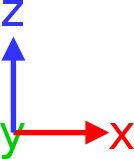
\includegraphics[width=0.04\textwidth]{Data/Images/Axes.png}};
			%%%%%
			\node[anchor=south west,inner sep=0] (fig_Steps0) at ({(\textwidth-\textwidth/10)*0.00+\textwidth/20},0){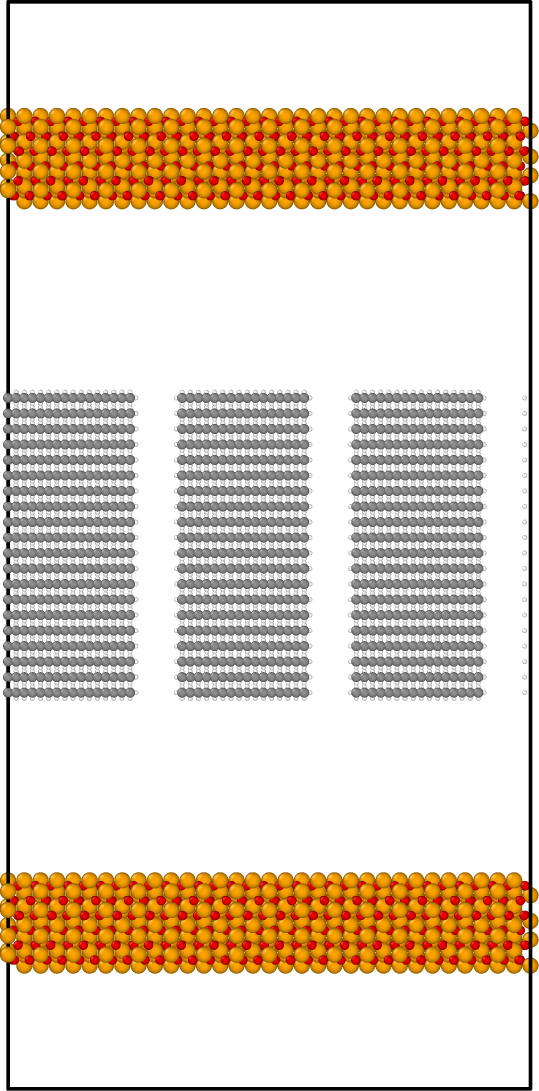
\includegraphics[width=0.150\textwidth]{Data/Images/1_initial.png}};
    			\support{3}{{(\textwidth-\textwidth/10)*0.00+\textwidth/20+\textwidth/24},					\textwidth/31};
    			\support{3}{{(\textwidth-\textwidth/10)*0.00+\textwidth/20+\textwidth/24+0.0669*\textwidth},	\textwidth/31};
    			\support{3}{{(\textwidth-\textwidth/10)*0.00+\textwidth/20+\textwidth/24},					0.278\textwidth}[180];
    			\support{3}{{(\textwidth-\textwidth/10)*0.00+\textwidth/20+\textwidth/24+0.0669*\textwidth},	0.278\textwidth}[180];
			%%%%%
			\node[anchor=south west,inner sep=0] (fig_Steps1) at ({(\textwidth-\textwidth/10)*0.25+\textwidth/20},0){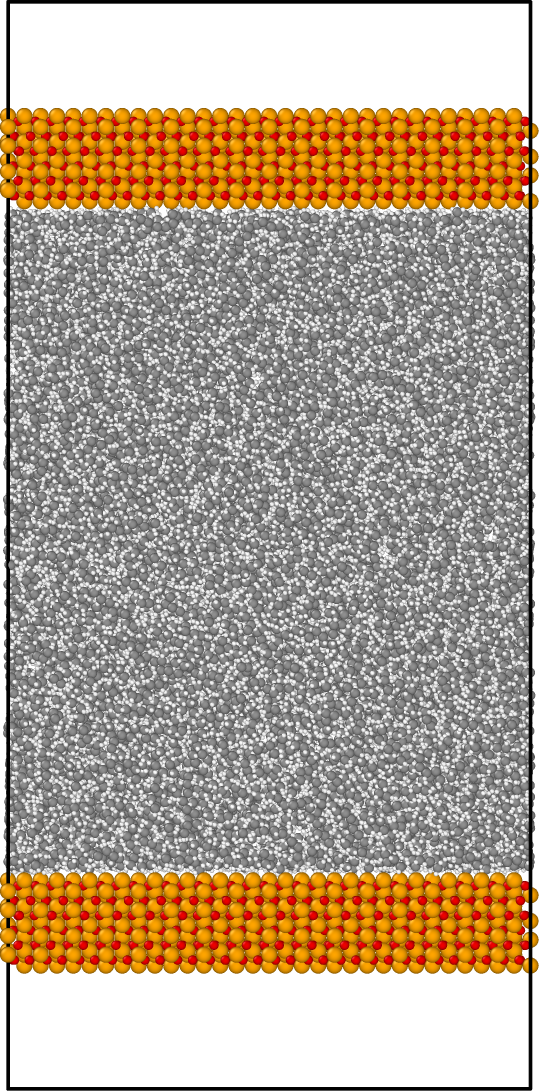
\includegraphics[width=0.150\textwidth]{Data/Images/2_equilibration.png}};
    			\support{3}{{(\textwidth-\textwidth/10)*0.25+\textwidth/20+\textwidth/24},					\textwidth/31};
    			\support{3}{{(\textwidth-\textwidth/10)*0.25+\textwidth/20+\textwidth/24+0.0669*\textwidth},	\textwidth/31};
    			\support{3}{{(\textwidth-\textwidth/10)*0.25+\textwidth/20+\textwidth/24},					0.278\textwidth}[180];
    			\support{3}{{(\textwidth-\textwidth/10)*0.25+\textwidth/20+\textwidth/24+0.0669*\textwidth},	0.278\textwidth}[180];
			%%%%%
			\node[anchor=south west,inner sep=0] (fig_Steps2) at ({(\textwidth-\textwidth/10)*0.50+\textwidth/20},0){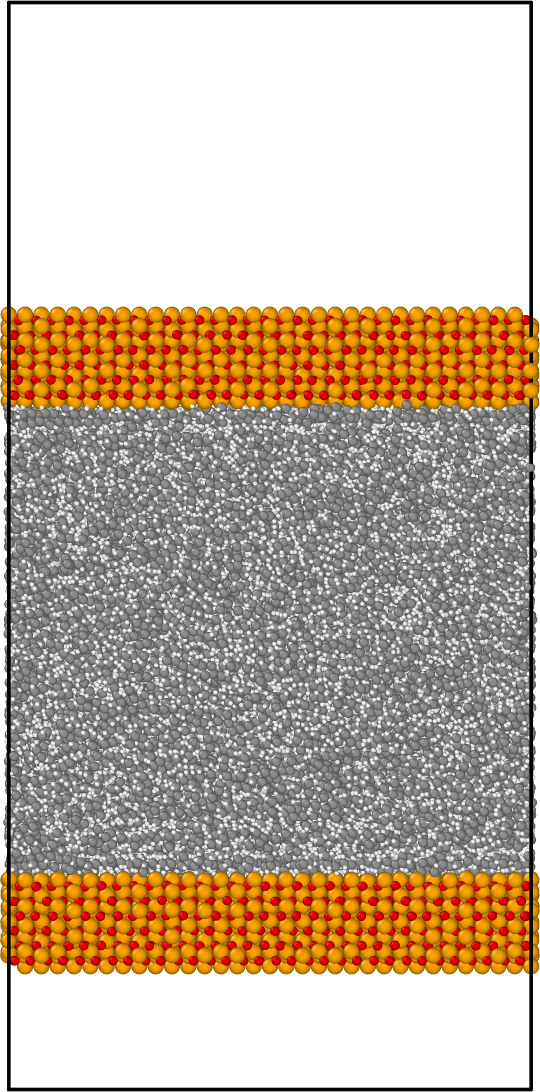
\includegraphics[width=0.150\textwidth]{Data/Images/3_Compression.png}};
    			\support{3}{{(\textwidth-\textwidth/10)*0.50+\textwidth/20+\textwidth/24},						\textwidth/31};
    			\support{3}{{(\textwidth-\textwidth/10)*0.50+\textwidth/20+\textwidth/24+0.0669*\textwidth},		\textwidth/31};
			\lineload{1}	{{(\textwidth-\textwidth/10)*0.50+\textwidth/20+\textwidth/110},					0.21*\textwidth}
						{{(\textwidth-\textwidth/10)*0.50+\textwidth/20+\textwidth/110+0.0669*2*\textwidth},	0.21*\textwidth}[0.5][0.5][0.11];
			\notation{5}{{(\textwidth-\textwidth/10)*0.50+\textwidth/20+\textwidth/110},					0.21*\textwidth}
						{{(\textwidth-\textwidth/10)*0.50+\textwidth/20+\textwidth/110+0.0669*2*\textwidth},	0.21*\textwidth}[$P$][][above left=0.077\linewidth];

			%%%%%
			\node[anchor=south west,inner sep=0] (fig_Steps3) at ({(\textwidth-\textwidth/10)*0.75+\textwidth/20},0){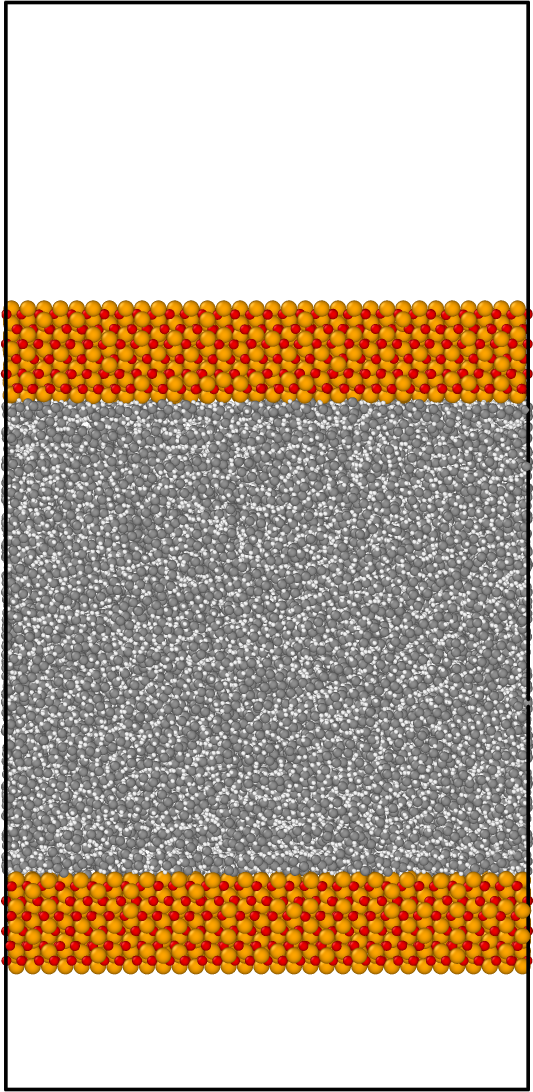
\includegraphics[width=0.148\textwidth]{Data/Images/4_shear.png}};
    			\support{4}{{(\textwidth-\textwidth/10)*0.75+\textwidth/20+\textwidth/24},						\textwidth/31};
    			\support{4}{{(\textwidth-\textwidth/10)*0.75+\textwidth/20+\textwidth/24+0.0669*\textwidth},		\textwidth/31};
			\lineload{1}	{{(\textwidth-\textwidth/10)*0.75+\textwidth/20+\textwidth/110},					0.21*\textwidth}
						{{(\textwidth-\textwidth/10)*0.75+\textwidth/20+\textwidth/110+0.0669*2*\textwidth},	0.21*\textwidth}[0.5][0.5][0.11];
			\notation{5}{{(\textwidth-\textwidth/10)*0.75+\textwidth/20+\textwidth/110},					0.21*\textwidth}
						{{(\textwidth-\textwidth/10)*0.75+\textwidth/20+\textwidth/110+0.0669*2*\textwidth},	0.21*\textwidth}[$P$][][above left=0.077\linewidth];
		
			\node (I) at (0.83*\textwidth, 0.206*\textwidth) {$\frac{v}{2}$} ;
			\node (J) at (0.78*\textwidth, 0.206*\textwidth) {} ;
			\draw [<- , line width=0.006*\textwidth] (I) -- (J);

			\node (K) at (0.78*\textwidth, 0.0455*\textwidth) {$\frac{v}{2}$} ;
			\node (L) at (0.83*\textwidth, 0.0455*\textwidth) {} ;
			\draw [<- , line width=0.006*\textwidth] (K) -- (L);
			

			\filldraw[fill=SERorange, draw=black] 	(0,4.5) circle (0.6125*3/4) node {Fe};
			\filldraw[fill=SERred, draw=black]  		(0,3.5) circle (0.365*3/4) node {O};
			\filldraw[fill=SERgray, draw=black]  		(0,2.5) circle (0.385*3/4) node {C};
			\filldraw[fill=SERwhite, draw=black]  	(0,1.5) circle (0.185) node {H};


			\begin{scope}[x={(fig_Steps0.south east)},y={(fig_Steps0.north west)}]
				\draw [](0.12\textwidth,-0.05) node[]{a)}	;
				\draw [](0.12\textwidth+0.225\textwidth,-0.05) node[]{b)}	;
				\draw [](0.12\textwidth+0.45\textwidth,-0.05) node[]{c)}	;
				\draw [](0.12\textwidth+0.675\textwidth,-0.05) node[]{d)}	;

			\end{scope}
		\end{tikzpicture}

		\caption{General steps carried out for the preparation and NEMD simulation of   each of the the systems considered in the present work. The orange atoms represent iron (Fe), the red ones oxygen (O), the gray ones carbon (C), and the white ones hydrogen (H). a) System generation. b) Equilibration. c) Compression. d) Shear. }
		\label{fig:Steps}
	\end{center}
\end{figure*}

\subsection{Equilibration}

First, alkane molecules were inserted between the slabs in an ordered fashion (Figure \ref{fig:Steps}a), followed by energy minimisation. Next, a properly equilibrated system was a generated using a simple 'brute force' scheme. In this procedure, the initially (artificially) ordered alkanes are heated to \SI{2000}{\kelvin} to accelerate diffusion, and left to evolve until equilibrium is reached (\SI{10}{\nano\second}). The system is then quenched back to the simulation temperature \SI{353}{\kelvin} over a further \SI{10}{\nano\second}. During the heat-quench sequence, the fluid temperature is controlled using a global Langevin thermostat \cite{Schneider1978} with a damping constant of \SI{0.1}{\pico\second} acting in all directions.

Three different criteria are considered to ensure that the systems have reached equilibrium. The first two, consist on verifying that there is convergence of the mean squared end-to-end distance $\left(\left< R^2 \right> \right)$ and of the mean squared radius of gyration $\left(\left< S^2 \right> \right)$. The final equilibrated configurations are taken as inputs for use in the following compression and shear simulations. The detailed procedure followed to equilibrate the systems can be found in the Appendix.

\subsection{Compression}

After the systems are properly equilibrated, the pressure was increased by giving a uniform normal force to the outer layer of Fe atoms in the top wall while keeping the outer layer of atoms in the bottom wall fixed in the z direction (see Figure \ref{fig:Regions}). Three different pressure values are considered here, namely \SI{0.5}{\giga\pascal}, \SI{1.0}{\giga\pascal} and \SI{1.5}{\giga\pascal}. These are of direct relevance to the EHL regime\cite{Spikes2014}.

\begin{figure}
    	\begin{center}
		\begin{tikzpicture}
			\node[anchor=south west,inner sep=0] (fig_regions) at (0,0){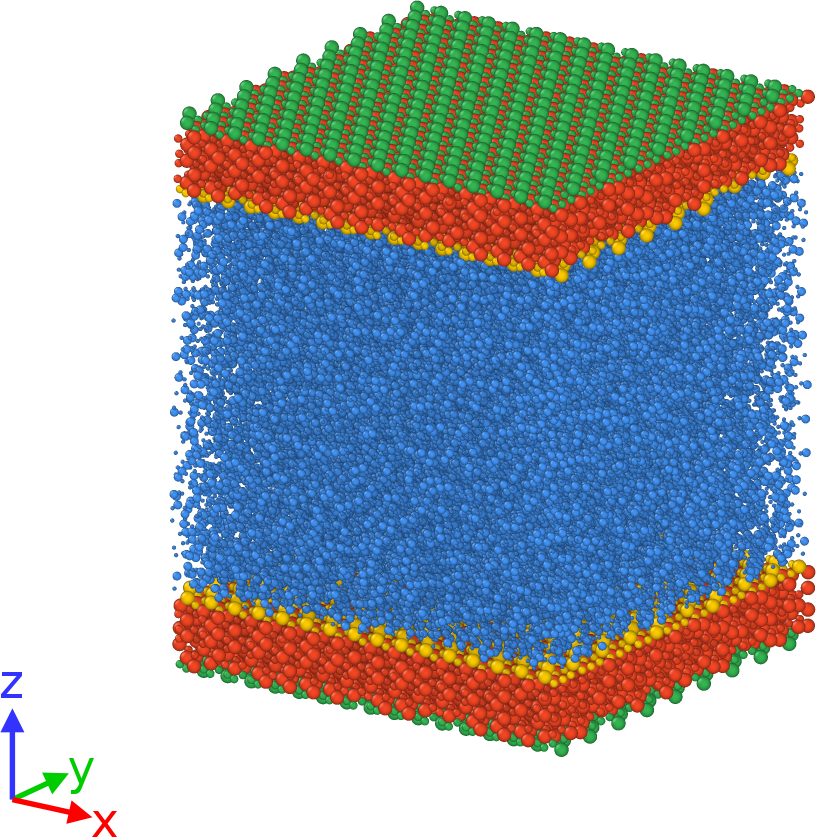
\includegraphics[width=0.25\textwidth]{Data/Images/5_region.png}};
			\begin{scope}[x={(fig_regions.south east)},y={(fig_regions.north west)}]
				\draw [](0,0.8) node[text width=1cm,align=center]{Top\\Wall}	;
				\draw [](0,0.53) node[]{Fluid}	;
				\draw [](0,0.27) node[text width=1cm,align=center]{Bottom\\Wall}	;

				\draw [decorate,decoration={brace}] (0.17,0.76) -- (0.17,0.86);
				\draw [decorate,decoration={brace}] (0.17,0.295) -- (0.17,0.755);
				\draw [decorate,decoration={brace}] (0.17,0.19) -- (0.17,0.29);

				\node (A) at (0.6,0.9) {} ;
				\node (B) at (1.0,1.0) [SERgreen]{Frozen} ;
				\draw [SERgreen, <- , line width=0.006*\textwidth] (A) -- (B);

				\node (C) at (0.8,0.78) {} ;
				\node (D) at (1.2,0.9) [SERorange2] {Thermostat} ;
				\draw [SERorange2, <- , line width=0.006*\textwidth] (C) -- (D);

				\node (E) at (0.8,0.74) {} ;
				\node (F) at (1.2,0.7) [SERyellow]{Free} ;
				\draw [SERyellow, <- , line width=0.006*\textwidth] (E) -- (F);
			\end{scope}
		\end{tikzpicture}
		\caption{Structure and regions of a typical system for the simulation of confined lubricants. The system is divided in three regions, namely, the fluid, and the top and bottom walls. Within each wall, the \textit{frozen} atoms (green) are used to apply the shearing and compressive constraints, and  the \textit{thermostat} atoms (orange) to control the temperature. Both the \textit{free} (yellow) and fluid (blue) atoms are left unconstrained.}
		\label{fig:Regions}
	\end{center}
\end{figure}

For the compression and shearing stages, the temperature of the system is controlled (T = \SI{353}{\kelvin}) by a Langevin thermostat \cite{Schneider1978} with a damping constant of \SI{0.1}{\pico\second} acting only on the central surface atoms (\textit{thermostat} in Figure \ref{fig:Regions}). The thermostat was applied only in the direction perpendicular to both the sliding and compression (\emph{y}). This approach is known to be more physically accurate than applying the thermostat directly to the confined fluid, which has been shown to significantly affect its behaviour under sliding conditions \cite{Liem1992,Bernardi2010,Yong2013}.

The compression phase is performed in two steps: first, the pressure is linearly incremented over \SI{10}{\nano\second} and then the target pressure is maintained for a further \SI{10}{\nano\second}. The density of the fluid region and the average pressure reach equilibrium well within the simulation time. The different final densities are presented in Table \ref{tab:rho} which correspond to the average density of the final \SI{1}{\nano\second} of the compression phase. In agreement with the available experimental data\cite{Griesbaum2000}, there is a clear increase in density with increasing alkane chain length as well as with increasing pressure.

\begin{table}
	\caption{Measured density values for confined alkanes  with three different chain lengths (C16, C30 and C60) at three different pressures (\SI{0.5}{\giga\pascal}, \SI{1.0}{\giga\pascal} and \SI{1.5}{\giga\pascal}).}   
	\centering     
	\begin{tabular}{c | l l  l}
		\hline\hline\\ [-2ex]

		
										&	\multicolumn{3}{c}{ $\rho \, [\SI{}{\kilogram\per\cubic\meter}]$} \\

		\hline\\ [-2ex]
		\backslashbox{Chain \\ Length}{P $[\SI{}{\giga\pascal}]$}	&	0.5		&	1.0		&	1.5	\\

		\hline\\ [-2ex]
		16C								&	0.87	&	0.93	&	0.98	\\
		30C								&	0.90	&	0.96	&	1.00	\\	
		60C								&	0.91	&	0.97	&	1.01	\\	

		\hline\hline    \\[-2ex]
	\end{tabular}
	\label{tab:rho}  
\end{table}

\subsection{Shear}

After the alkane chains are fully equilibrated at the target pressures (\SI{0.5}{\giga\pascal}, \SI{1.0}{\giga\pascal}, \SI{1.5}{\giga\pascal}), the shear response of the lubricant is studied. A shear velocity gradient was imposed on the system by means of a constant velocity, $v_x = \pm v_s/2$ applied to the outermost layer of atoms in each slab (see Figure \ref{fig:Steps}) in the \emph{x} direction. We consider the following sliding velocities, $v_s$; \SI{10}{\meter\per\second}, \SI{20}{\meter\per\second}, \SI{50}{\meter\per\second} and \SI{100}{\meter\per\second}. For the simulated film thickness (approx. \SI{80}{\nano\meter}), these correspond to shear rates of approximately $10^{9} - 10^{10} s^{-1}$. While these are above those encountered in real engineering components \cite{Taylor2017}, lower shear rates do not reach a steady state in the available simulation time\cite{Ewen2018}.

To verify that a nonequilibrium steady state was reached, the evolution of the RMS end-to-end distance $\left(\left< R^2 \right> \right)$, the segmental orientation $\left(\left<P_{2}^{xz} \right> \right)$ and the shear stress $\left(F_L \right)$ on the surfaces in response to the fluid, were monitored. Lower sliding velocities require a longer simulation time to reach a steady state; however, they require a similar sliding distance, as observed experimentally~\cite{Drummond2000}. In general, a steady state is reached in a shorter sliding distance for shorter alkanes and lower pressures. A representative case is C30 at \SI{1.0}{\giga\pascal}, for which the evolution of the end-to-end distance, segmental orientation, and shear stress are presented at four sliding velocities in Figure \ref{fig:SS}.

% \pgfmathsetmacro{\SERFigwidth}{.035\linewidth}
% \pgfmathsetmacro{\SERFigheight}{.036\linewidth}
% \begin{figure}
%     	\begin{center}
% 		\begin{gnuplot}[terminal=pdf, terminaloptions={size \SERFigwidth cm, \SERFigheight cm color solid}]
% 			set multiplot layout 4,1 rowsfirst
% 			set format x ' '
% 			unset xlabel

% 			set key bottom right
% 			set key samplen  0.0
% 			set ylabel "$\\left< R^2\\right>  \\,[\\SI{}{\\square\\angstrom}]$"          
% 			set label at graph 0.03,0.89 left "a)"
% 			set lmargin at screen 0.25; set rmargin at screen 0.9
% 			set tmargin at screen 1.00; set bmargin at screen 0.775
% 			set ytics 280,40,400 
% 			plot [:1100][260:440] 	'Data/Shear/C30/1.0GPa/10m_s/e2e2.plot_s.plot'  u  (($1/1e6)*10):($2) lt 3 pt 3 notitle  , 'Data/Shear/C30/1.0GPa/10m_s2/e2e2.plot_s.plot'  u (($1/1e6)*10):($2)  lt 3 pt 3 notitle ,\
% 								'Data/Shear/C30/1.0GPa/20m_s/e2e2.plot_s.plot'  u  (($1/1e6)*20):($2) lt 4 pt 4 notitle  , 'Data/Shear/C30/1.0GPa/20m_s2/e2e2.plot_s.plot'  u (($1/1e6)*20):($2)  lt 4 pt 4 notitle ,\
% 								'Data/Shear/C30/1.0GPa/50m_s/e2e2.plot_s.plot'   u (($1/1e6)*50):($2) lt 5 pt 5 notitle  , 'Data/Shear/C30/1.0GPa/50m_s2/e2e2.plot_s.plot' u  (($1/1e6)*50):($2)  lt 5 pt 5 notitle ,\
% 								'Data/Shear/C30/1.0GPa/100m_s/e2e2.plot_s.plot' u  (($1/1e6)*100):($2) lt 10 pt 10 notitle  , 'Data/Shear/C30/1.0GPa/100m_s2/e2e2.plot_s.plot' u (($1/1e6)*100):($2) lt 10 pt 10  notitle 
			
% 			unset label
% 			set tmargin at screen 0.775; set bmargin at screen 0.550
% 			set ytics 0.3, 0.1, 0.5			
% 			set ylabel "$\\left<P_{2}^{xz}\\right>$"        
% 			set label at graph 0.03,0.89 left "b)"  
% 			plot  [:1100][0.25:0.6]	'Data/Shear/C30/1.0GPa/10m_s/P2XZ_s.plot' u   (($1/1e6)*10):($2) lt 3 pt 3 title '' , 'Data/Shear/C30/1.0GPa/10m_s2/P2XZ_s.plot' u   (($1/1e6)*10):($2) lt 3 pt 3 notitle  ,\
% 								'Data/Shear/C30/1.0GPa/20m_s/P2XZ_s.plot' u   (($1/1e6)*20):($2) lt 4 pt 4 title '' , 'Data/Shear/C30/1.0GPa/20m_s2/P2XZ_s.plot' u   (($1/1e6)*20):($2) lt 4 pt 4 notitle  ,\
% 								'Data/Shear/C30/1.0GPa/50m_s/P2XZ_s.plot' u  (($1/1e6)*50):($2)  lt 5 pt 5 title '' , 'Data/Shear/C30/1.0GPa/50m_s2/P2XZ_s.plot' u  (($1/1e6)*50):($2)  lt 5 pt 5 notitle ,\
% 								'Data/Shear/C30/1.0GPa/100m_s/P2XZ_s.plot' u  (($1/1e6)*100):($2) lt 10 pt 10 title '' , 'Data/Shear/C30/1.0GPa/100m_s2/P2XZ_s.plot' u (($1/1e6)*100):($2) lt 10 pt 10 notitle 

% 			unset label
% 			set tmargin at screen 0.550; set bmargin at screen 0.325
% 			set ytics 30, 30, 120 
% 			set ylabel "$F_L \\, [\\SI{}{\\mega\\pascal}]$"          
% 			set label at graph 0.03,0.89 left "c)"
% 			plot  [:1100][20:150]	'Data/Shear/C30/1.0GPa/10m_s/fc_ave.dump.plot' u (($1/1e6)*10):($2/10)  lt 3 pt 3 notitle  , 'Data/Shear/C30/1.0GPa/10m_s2/fc_ave.dump.plot' u (($1/1e6)*10):($2/10)   lt 3 pt 3 notitle   ,\
% 							'Data/Shear/C30/1.0GPa/20m_s/fc_ave.dump.plot' u (($1/1e6)*20):($2/10)  lt 4 pt 4 notitle  , 'Data/Shear/C30/1.0GPa/20m_s2/fc_ave.dump.plot' u (($1/1e6)*20):($2/10)   lt 4 pt 4 notitle   ,\
% 							'Data/Shear/C30/1.0GPa/50m_s/fc_ave.dump.plot' u (($1/1e6)*50):($2/10)   lt 5 pt 5 notitle  , 'Data/Shear/C30/1.0GPa/50m_s2/fc_ave.dump.plot'  u (($1/1e6)*50):($2/10)  lt 5 pt 5 notitle  ,\
% 							'Data/Shear/C30/1.0GPa/100m_s/fc_ave.dump.plot' u (($1/1e6)*100):($2/10) lt 10 pt 10 notitle  , 'Data/Shear/C30/1.0GPa/100m_s2/fc_ave.dump.plot'  u (($1/1e6)*100):($2/10) lt 10 pt 10 notitle  

% 			unset label
% 			set format x '%g'
% 			set xlabel "Distance [\\SI{}{\\nano\\meter}]"  
% 			set tmargin at screen 0.325; set bmargin at screen 0.10
% 			#set label at graph 1.01,0.1 left "$\\times 10^{6}$"
% 			set ytics 300,100,700
% 			set ylabel "$T \\, [\\SI{}{\\kelvin}]$"          
% 			set label at graph 0.03,0.89 left "d)"
% 			plot  [:1100][280:750] 	'<grep c_temp_fluid Data/Shear/C30/1.0GPa/10m_s/log.comp_shear.plot'     u (($0/1000)*10):($6)        lt 3    pt 3    notitle ,\
% 								'<grep temp_flu Data/Shear/C30/1.0GPa/10m_s2/log.comp_shear.plot'   u (($0/1000+20)*10):($6) lt 3    pt 3    title  "\\SI{10}{\\meter\\per\\second}" ,\
% 								'<grep c_temp_fluid Data/Shear/C30/1.0GPa/20m_s/log.comp_shear.plot'     u (($0/1000)*20):($6)        lt 4    pt 4    notitle ,\
% 								'<grep c_temp_fluid Data/Shear/C30/1.0GPa/20m_s2/log.comp_shear.plot'   u (($0/1000+10)*20):($6) lt 4    pt 4    title  "\\SI{20}{\\meter\\per\\second}" ,\
% 								'<grep c_temp_fluid Data/Shear/C30/1.0GPa/50m_s/log.comp_shear.plot'     u (($0/1000)*50):($6)        lt 5    pt 5    notitle ,\
% 								'<grep c_temp_fluid Data/Shear/C30/1.0GPa/50m_s2/log.comp_shear.plot'   u (($0/1000+5)*50):($6)   lt 5    pt 5     title  "\\SI{50}{\\meter\\per\\second}" ,\
% 								'<grep c_temp_fluid Data/Shear/C30/1.0GPa/100m_s/log.comp_shear.plot'   u (($0/1000)*100):($6)     lt 10  pt 10   notitle ,\
% 								'<grep c_temp_fluid Data/Shear/C30/1.0GPa/100m_s2/log.comp_shear.plot' u (($0/1000+5)*100):($6) lt 10  pt 10  title  "\\SI{100}{\\meter\\per\\second}"
% 			unset multiplot
% 		\end{gnuplot}

% 		\caption{Evolution of the a) mean squared end-to-end distance $\left(\left< R^2 \right>\right)$, b) the average segmental orientation  $\left(\left<P_{2}^{xz}\right>\right)$, c) the lateral (friction) force  $\left(F_L\right)$ and d) the temperature $\left(T\right)$ for a system with alkane chains of length C30 at a pressure of \SI{1.0}{\giga\pascal} and  three  shearing velocities. The transient state begins with the application of the shear displacement of the surfaces and ends when  steady state is attained. Note that $1 \times 10^{6}$ steps correspond to \SI{1}{\nano\second}.}
% 		\label{fig:SSOLD}
% 	\end{center}
%  \end{figure}
 
 
 
 
 
\pgfmathsetmacro{\SERFigwidth}{.035\linewidth}
\pgfmathsetmacro{\SERFigheight}{.036\linewidth}
\begin{figure}
    	\begin{center}
		\begin{gnuplot}[terminal=pdf, terminaloptions={size \SERFigwidth cm, \SERFigheight cm color solid}]
			set multiplot layout 4,1 rowsfirst
			set format x ' '
			unset xlabel
			set key top right
			set key samplen  0.0
			set ylabel "$\\left< R^2\\right>  \\,[\\SI{}{\\square\\angstrom}]$"          
			set label at graph 0.03,0.89 left "a)"
			set lmargin at screen 0.25; set rmargin at screen 0.9
			set tmargin at screen 1.00; set bmargin at screen 0.7
			set ytics 280,40,400 
			plot [:600][260:440] 	'Data/Shear/C30/1.0GPa/10m_s/e2e2.plot_s.plot'  u  (($1/1e6)*10):($2) lt 3 pt 3 notitle  , 'Data/Shear/C30/1.0GPa/10m_s2/e2e2.plot_s.plot'  u (($1/1e6)*10):($2)  lt 3 pt 3 notitle ,\
								'Data/Shear/C30/1.0GPa/20m_s/e2e2.plot_s.plot'  u  (($1/1e6)*20):($2) lt 4 pt 4 notitle  , 'Data/Shear/C30/1.0GPa/20m_s2/e2e2.plot_s.plot'  u (($1/1e6)*20):($2)  lt 4 pt 4 notitle ,\
								'Data/Shear/C30/1.0GPa/50m_s/e2e2.plot_s.plot'   u (($1/1e6)*50):($2) lt 5 pt 5 notitle  , 'Data/Shear/C30/1.0GPa/50m_s2/e2e2.plot_s.plot' u  (($1/1e6)*50):($2)  lt 5 pt 5 notitle ,\
								'Data/Shear/C30/1.0GPa/100m_s/e2e2.plot_s.plot' u  (($1/1e6)*100):($2) lt 10 pt 10 notitle  , 'Data/Shear/C30/1.0GPa/100m_s2/e2e2.plot_s.plot' u (($1/1e6)*100):($2) lt 10 pt 10  notitle 
			
			unset label
			set tmargin at screen 0.7; set bmargin at screen 0.4
			set ytics 0.3, 0.1, 0.6			
			set ylabel "$\\left<P_{2}^{xz}\\right>$"        
			set label at graph 0.03,0.89 left "b)"  
			plot  [:600][0.28:0.65]	'Data/Shear/C30/1.0GPa/10m_s/P2XZ_s.plot' u   (($1/1e6)*10):($2) lt 3 pt 3 title '' , 'Data/Shear/C30/1.0GPa/10m_s2/P2XZ_s.plot' u   (($1/1e6)*10):($2) lt 3 pt 3 notitle  ,\
								'Data/Shear/C30/1.0GPa/20m_s/P2XZ_s.plot' u   (($1/1e6)*20):($2) lt 4 pt 4 title '' , 'Data/Shear/C30/1.0GPa/20m_s2/P2XZ_s.plot' u   (($1/1e6)*20):($2) lt 4 pt 4 notitle  ,\
								'Data/Shear/C30/1.0GPa/50m_s/P2XZ_s.plot' u  (($1/1e6)*50):($2)  lt 5 pt 5 title '' , 'Data/Shear/C30/1.0GPa/50m_s2/P2XZ_s.plot' u  (($1/1e6)*50):($2)  lt 5 pt 5 notitle ,\
								'Data/Shear/C30/1.0GPa/100m_s/P2XZ_s.plot' u  (($1/1e6)*100):($2) lt 10 pt 10 title '' , 'Data/Shear/C30/1.0GPa/100m_s2/P2XZ_s.plot' u (($1/1e6)*100):($2) lt 10 pt 10 notitle 

			unset label
			set tmargin at screen 0.4; set bmargin at screen 0.1
			set ytics 30, 30, 120 
			set ylabel "$F_L \\, [\\SI{}{\\mega\\pascal}]$" 
			set format x '%g'
			set xlabel "Distance [\\SI{}{\\nano\\meter}]"  

			set label at graph 0.03,0.89 left "c)"
			plot  [:600][40:150]	'Data/Shear/C30/1.0GPa/10m_s/fc_ave.dump.plot' u (($1/1e6)*10):($2/10)  lt 3 pt 3 notitle  ,                           'Data/Shear/C30/1.0GPa/10m_s2/fc_ave.dump.plot' u (($1/1e6)*10):($2/10)   lt 3 pt 3 title  "\\SI{10}{\\meter\\per\\second}"   ,\
							'Data/Shear/C30/1.0GPa/20m_s/fc_ave.dump.plot' u (($1/1e6)*20):($2/10)  lt 4 pt 4 notitle  , 'Data/Shear/C30/1.0GPa/20m_s2/fc_ave.dump.plot' u (($1/1e6)*20):($2/10)   lt 4 pt 4 title  "\\SI{20}{\\meter\\per\\second}"   ,\
							'Data/Shear/C30/1.0GPa/50m_s/fc_ave.dump.plot' u (($1/1e6)*50):($2/10)   lt 5 pt 5 notitle  , 'Data/Shear/C30/1.0GPa/50m_s2/fc_ave.dump.plot'  u (($1/1e6)*50):($2/10)  lt 5 pt 5 title  "\\SI{50}{\\meter\\per\\second}"  ,\
							'Data/Shear/C30/1.0GPa/100m_s/fc_ave.dump.plot' u (($1/1e6)*100):($2/10) lt 10 pt 10 notitle  , 'Data/Shear/C30/1.0GPa/100m_s2/fc_ave.dump.plot'  u (($1/1e6)*100):($2/10) lt 10 pt 10 title  "\\SI{100}{\\meter\\per\\second}"  

			unset multiplot
		\end{gnuplot}

		\caption{Evolution of the a) mean squared end-to-end distance $\left(\left< R^2 \right>\right)$, b) the average segmental orientation  $\left(\left<P_{2}^{xz}\right>\right)$, c) the lateral (friction) force  $\left(F_L\right)$ and d) the temperature $\left(T\right)$ for a system with alkane chains of length C30 at a pressure of \SI{1.0}{\giga\pascal} and  three  shearing velocities. The transient state begins with the application of the shear displacement of the surfaces and ends when  steady state is attained. Note that $1 \times 10^{6}$ steps correspond to \SI{1}{\nano\second}.}
		\label{fig:SS}
	\end{center}
 \end{figure}


Since the initial configuration is the same for all of the shearing velocities, they all have an initial value of $\left< R^2 \right> = \SI{283}{\angstrom\squared}$. After this point, $\left< R^2 \right> $ increases and then asymptotes towards a steady state value. This suggests that the chains generally unfold when shear is applied. The steady state $\left< R^2 \right>$ is lower at higher sliding velocity, as has been observed in previous simulations of similar systems at high shear rates\cite{Cho2017}. This decrease has been ascribed to strong intermolecular collisions together with intense chain rotation and tumbling dynamics at high shear rates.

For ideal chains in the bulk, the average segmental orientation, $\langle P_{2}^{xz}\rangle=0.25$. This value is obtained by assuming an uniform distribution of the orientation of the bonds, which corresponds to having an average orientation of \SI{45}{\degree}. When under confinement, polymer chains close to the surfaces tend to lye parallel to them (the angle formed between the chain and the surface is close to zero) generating a natural increase in the value of  $\langle P_{2}^{xz}\rangle$.

In the case of C30 at \SI{1.0}{\giga\pascal}, $\langle P_{2}^{xz}\rangle=0.32$ before shear is applied (see Figure \ref{fig:SS}b), indicating that there is a preferential orientation caused by the presence of the surfaces. When sliding is initiated, the chains begin to align with the flow direction, increasing $\langle P_{2}^{xz}\rangle$.

% Sebastian - What about P_{2}^{xy}? This is should be directly proportional to friction for bulk sheared polymers (see Jeong2017)

The shear stress was monitored through the average lateral (friction) force $F_L$ acting on the outermost layer of atoms (frozen atoms in Figure \ref{fig:Regions}) in the top and bottom slabs (divided by their area) in response to the fluid. At the onset of sliding, $F_L$ increases rapidly to reach a maximum value and then decreases before reaching a steady state, indicating stress overshoot behaviour\cite{Jeong2017}. The sliding distance needed for $F_L$ to reach a steady state is consistent with that needed for $\left< R^2 \right> $ and $\left<P_{2}^{xz} \right> $ (Figure \ref{fig:SS}).

Once the simulations reach a steady state (Figure \ref{fig:SS}), they are run for \SI{5}{\nano\second} to \SI{20}{\nano\second} while maintaining constant the shearing velocity and the applied pressure. During the final \SI{2}{\nano\second} of the simulation, $\left(\left< R^2 \right> \right)$, $\left<P_{2}^{xz} \right> $, and $\left(F_L\right)$ are measured and averaged; the results and analysis of these measurements are presented in the next section.

%%%%%%%%%%%%%%%%%%%%%%%%%%%%%%%%%%%%%%%%%%%%%%%%%

\section{Results and Discussion}

\subsection{Chain extension and orientation}

Longer chains will clearly have a larger $\left< R^2 \right> $, so to compare the variation of $\left< R^2 \right> $ between the different chain lengths, the root mean squared end-to-end distance \emph{per bond}; $\left< R^2 \right>/\left(N_\text{bonds}\right)^2$, is presented as a function of shear rate in Figure \ref{fig:e2e2_v} for the different chain lengths and pressures studied.


 \pgfmathsetmacro{\SERFigwidth}{.035\linewidth}
\pgfmathsetmacro{\SERFigheight}{.026\linewidth}
\begin{figure}
    	\begin{center}
		\begin{gnuplot}[terminal=pdf, terminaloptions={size \SERFigwidth cm, \SERFigheight cm color solid}]
			set key above
			set xlabel  "$\\dot{\\gamma} \\, \\left[ \\SI{}{\\per\\second} \\right]$"  
			set ylabel "$\\left< R^2 \\right>/\\left(N_\\text{bonds}\\right)^2$ [\\SI{}{\\square\\angstrom}]"
			set ytics 0.3,0.1,0.6
			set key noautotitle
			set format x  '$10^{%L}$' 
			set logscale x
			p [:2e10][0.28:0.601]	'Data/Shear/Compiled_e2e2_v.plot8.plot' i 0 u ($3/($12*1e-10)):($6/($1-1)**2):($7/($1-1)**2) w errorbars title "$\\SI{0.5}{\\giga\\pascal}$" lt 1 lc 0 ps 1,\
				'Data/Shear/Compiled_e2e2_v.plot8.plot' i 1 u ($3/($12*1e-10)):($6/($1-1)**2):($7/($1-1)**2) w errorbars title  "$\\SI{1.0}{\\giga\\pascal}$" lt 2 lc 0 ps 1,\
				'Data/Shear/Compiled_e2e2_v.plot8.plot' i 1 u ($3/($12*1e-10)):($6/($1-1)**2) w l notitle lt 2 lc 1  lw 2 ,\
				'Data/Shear/Compiled_e2e2_v.plot8.plot' i 2 u ($3/($12*1e-10)):($6/($1-1)**2):($7/($1-1)**2) w errorbars title  "$\\SI{1.5}{\\giga\\pascal}$" lt 3 lc 0 ps 1,\
				'Data/Shear/Compiled_e2e2_v.plot8.plot' i 2 u ($3/($12*1e-10)):($6/($1-1)**2) w l notitle lt 3 lc 1 lw 2 ,\
				'Data/Shear/Compiled_e2e2_v.plot8.plot' i 3 u ($3/($12*1e-10)):($6/($1-1)**2):($7/($1-1)**2) w errorbars notitle lt 1 lc 0 ps 1 ,\
				'Data/Shear/Compiled_e2e2_v.plot8.plot' i 0 u ($3/($12*1e-10)):($6/($1-1)**2) w l title "C16" lt 1 lc 1 lw 2 ,\
				'Data/Shear/Compiled_e2e2_v.plot8.plot' i 3 u ($3/($12*1e-10)):($6/($1-1)**2) w l title "C30" lt 1 lc 2 lw 2 ,\				
				'Data/Shear/Compiled_e2e2_v.plot8.plot' i 4 u ($3/($12*1e-10)):($6/($1-1)**2) w l notitle lt 2 lc 2 lw 2 ,\
				'Data/Shear/Compiled_e2e2_v.plot8.plot' i 4 u ($3/($12*1e-10)):($6/($1-1)**2):($7/($1-1)**2) w errorbars notitle lt 2 lc 0 ps 1,\
				'Data/Shear/Compiled_e2e2_v.plot8.plot' i 5 u ($3/($12*1e-10)):($6/($1-1)**2) w l notitle lt 3 lc 2 lw 2 ,\
				'Data/Shear/Compiled_e2e2_v.plot8.plot' i 5 u ($3/($12*1e-10)):($6/($1-1)**2):($7/($1-1)**2) w errorbars notitle lt 3 lc 0 ps 1 ,\
				'Data/Shear/Compiled_e2e2_v.plot8.plot' i 6 u ($3/($12*1e-10)):($6/($1-1)**2):($7/($1-1)**2) w errorbars notitle lt 1 lc 0 ps 1 ,\
				'Data/Shear/Compiled_e2e2_v.plot8.plot' i 6 u ($3/($12*1e-10)):($6/($1-1)**2) w l title 'C60' lt 1 lc 3 lw 2 ,\				
				'Data/Shear/Compiled_e2e2_v.plot8.plot' i 7 u ($3/($12*1e-10)):($6/($1-1)**2) w l notitle  lt 2 lc 3 lw 2 ,\
				'Data/Shear/Compiled_e2e2_v.plot8.plot' i 7 u ($3/($12*1e-10)):($6/($1-1)**2):($7/($1-1)**2) w errorbars notitle  lt 2 lc 0 ps 1,\
				'Data/Shear/Compiled_e2e2_v.plot8.plot' i 8 u ($3/($12*1e-10)):($6/($1-1)**2) w l notitle  lt 3 lc 3 lw 2 ,\
				'Data/Shear/Compiled_e2e2_v.plot8.plot' i 8 u ($3/($12*1e-10)):($6/($1-1)**2):($7/($1-1)**2) w errorbars notitle  lt 3 lc 0 ps 1,\
		\end{gnuplot}
		\caption{Average squared end-to-end distance per bond as a function of the shear rate $\left( \dot{\gamma} \right)$ measured after reaching steady state.}
		\label{fig:e2e2_v}
	\end{center}
 \end{figure}
 
 
Generally, for the chain lengths and pressures studied, $\left< R^2 \right>/\left(N_\text{bonds}\right)^2$ decreases with increasing shear rate, suggesting more compact chain conformations. This has been observed in previous simulations of similar systems at high shear rates\cite{Cho2017}. This decrease has been ascribed to stronger intermolecular collisions together with intense chain rotation and tumbling dynamics at high shear rates. Longer chains at higher pressures are relatively less extended than shorter chains at lower pressures.

There is also a reduction of $\left<P_{2}^{xz} \right> $ with increasing shear rate for all the considered chain lengths and pressures (see Figure \ref{fig:P2_v}). This indicates an increase of the average angle of segments relative to the shearing direction at higher shear rate, meaning that the chains are less aligned with shearing direction.
% Are we sure? Would expect the reverse to be true... Need citation and explanation (maybe 'Fluid n-decane undergoing planar Couette flow')
Longer chains tend be more aligned with the shearing direction, whereas the chains are less aligned at higher pressure.

\pgfmathsetmacro{\SERFigwidth}{.035\linewidth}
\pgfmathsetmacro{\SERFigheight}{.026\linewidth}
\begin{figure}
    	\begin{center}
		\begin{gnuplot}[terminal=pdf, terminaloptions={size \SERFigwidth cm, \SERFigheight cm color solid}]
			set key above
			set xlabel  "$\\dot{\\gamma} \\, \\left[ \\SI{}{\\per\\second} \\right]$"  
			set ylabel "$\\left<P_{2}^{xz}\\right>$"
			set key noautotitle
			set format x  '$10^{%L}$' 
			set logscale x
			p [:2e10][]	'Data/Shear/Compiled_e2e2_v.plot8.plot' i 0 u ($3/($12*1e-10)):($8) title "$\\SI{0.5}{\\giga\\pascal}$" lt 1 lc 0 ps 1,\
					'Data/Shear/Compiled_e2e2_v.plot8.plot' i 1 u ($3/($12*1e-10)):($8) title  "$\\SI{1.0}{\\giga\\pascal}$" lt 2 lc 0 ps 1,\
					'Data/Shear/Compiled_e2e2_v.plot8.plot' i 1 u ($3/($12*1e-10)):($8) w l notitle lt 2 lc 1  lw 2 ,\
					'Data/Shear/Compiled_e2e2_v.plot8.plot' i 2 u ($3/($12*1e-10)):($8) title  "$\\SI{1.5}{\\giga\\pascal}$" lt 3 lc 0 ps 1,\
					'Data/Shear/Compiled_e2e2_v.plot8.plot' i 2 u ($3/($12*1e-10)):($8) w l notitle lt 3 lc 1 lw 2 ,\
					'Data/Shear/Compiled_e2e2_v.plot8.plot' i 3 u ($3/($12*1e-10)):($8) notitle lt 1 lc 0 ps 1 ,\
					'Data/Shear/Compiled_e2e2_v.plot8.plot' i 0 u ($3/($12*1e-10)):($8) w l title "C16" lt 1 lc 1 lw 2 ,\
					'Data/Shear/Compiled_e2e2_v.plot8.plot' i 3 u ($3/($12*1e-10)):($8) w l title "C30" lt 1 lc 2 lw 2 ,\				
					'Data/Shear/Compiled_e2e2_v.plot8.plot' i 4 u ($3/($12*1e-10)):($8) w l notitle lt 2 lc 2 lw 2 ,\
					'Data/Shear/Compiled_e2e2_v.plot8.plot' i 4 u ($3/($12*1e-10)):($8) notitle lt 2 lc 0 ps 1,\
					'Data/Shear/Compiled_e2e2_v.plot8.plot' i 5 u ($3/($12*1e-10)):($8) w l notitle lt 3 lc 2 lw 2 ,\
					'Data/Shear/Compiled_e2e2_v.plot8.plot' i 5 u ($3/($12*1e-10)):($8) notitle lt 3 lc 0 ps 1 ,\
					'Data/Shear/Compiled_e2e2_v.plot8.plot' i 6 u ($3/($12*1e-10)):($8) notitle lt 1 lc 0 ps 1 ,\
					'Data/Shear/Compiled_e2e2_v.plot8.plot' i 6 u ($3/($12*1e-10)):($8) w l title 'C60' lt 1 lc 3 lw 2 ,\				
					'Data/Shear/Compiled_e2e2_v.plot8.plot' i 7 u ($3/($12*1e-10)):($8) w l notitle  lt 2 lc 3 lw 2 ,\
					'Data/Shear/Compiled_e2e2_v.plot8.plot' i 7 u ($3/($12*1e-10)):($8) notitle  lt 2 lc 0 ps 1,\
					'Data/Shear/Compiled_e2e2_v.plot8.plot' i 8 u ($3/($12*1e-10)):($8) w l notitle  lt 3 lc 3 lw 2 ,\
					'Data/Shear/Compiled_e2e2_v.plot8.plot' i 8 u ($3/($12*1e-10)):($8) notitle  lt 3 lc 0 ps 1,\
		\end{gnuplot}
		\caption{Average segmental orientation as a function of the shear rate $\left( \dot{\gamma} \right)$ measured after reaching steady state. Error bars, calculated from the standard deviation between the trajectory time-averages, are omitted for clarity, but are of a similar size to the symbols.}
		\label{fig:P2_v}
	\end{center}
 \end{figure}

\subsection{Friction}

% \pgfmathsetmacro{\SERFigwidth}{.035\linewidth}
% \pgfmathsetmacro{\SERFigheight}{.026\linewidth}
% \begin{figure}
%     	\begin{center}
% 		\begin{gnuplot}[terminal=pdf, terminaloptions={size \SERFigwidth cm, \SERFigheight cm color solid}]
% 			set key above
% 			set xlabel  "x Velocity $\\left[ \\SI{}{\\meter\\per\\second} \\right]$"  
% 			set ylabel "$F_L \\, [\\SI{}{\\mega\\pascal}]$"
% 			set ytics 20,20,120
% 			set key noautotitle
% 			p [:110][15:125]	'Data/Shear/Compiled_e2e2_v.plot8.plot' i 0 u ($3):($4/10):($5/10) w p title "$\\SI{0.5}{\\giga\\pascal}$" lt 1 lc 0 ps 1,\
% 				'Data/Shear/Compiled_e2e2_v.plot8.plot' i 1 u ($3):($4/10):($5/10) w p title  "$\\SI{1.0}{\\giga\\pascal}$" lt 2 lc 0 ps 1,\
% 				'Data/Shear/Compiled_e2e2_v.plot8.plot' i 1 u ($3):($4/10) w l notitle lt 2 lc 1  lw 2 ,\
% 				'Data/Shear/Compiled_e2e2_v.plot8.plot' i 2 u ($3):($4/10):($5/10) w p title  "$\\SI{1.5}{\\giga\\pascal}$" lt 3 lc 0 ps 1,\
% 				'Data/Shear/Compiled_e2e2_v.plot8.plot' i 2 u ($3):($4/10) w l notitle lt 3 lc 1 lw 2 ,\
% 				'Data/Shear/Compiled_e2e2_v.plot8.plot' i 3 u ($3):($4/10):($5/10) w p notitle lt 1 lc 0 ps 1 ,\
% 				'Data/Shear/Compiled_e2e2_v.plot8.plot' i 0 u ($3):($4/10) w l title "C16" lt 1 lc 1 lw 2 ,\
% 				'Data/Shear/Compiled_e2e2_v.plot8.plot' i 3 u ($3):($4/10) w l title "C30" lt 1 lc 2 lw 2 ,\				
% 				'Data/Shear/Compiled_e2e2_v.plot8.plot' i 4 u ($3):($4/10) w l notitle lt 2 lc 2 lw 2 ,\
% 				'Data/Shear/Compiled_e2e2_v.plot8.plot' i 4 u ($3):($4/10):($5/10) w p notitle lt 2 lc 0 ps 1,\
% 				'Data/Shear/Compiled_e2e2_v.plot8.plot' i 5 u ($3):($4/10) w l notitle lt 3 lc 2 lw 2 ,\
% 				'Data/Shear/Compiled_e2e2_v.plot8.plot' i 5 u ($3):($4/10):($5/10) w p notitle lt 3 lc 0 ps 1 ,\
% 				'Data/Shear/Compiled_e2e2_v.plot8.plot' i 6 u ($3):($4/10):($5/10) w p notitle lt 1 lc 0 ps 1 ,\
% 				'Data/Shear/Compiled_e2e2_v.plot8.plot' i 6 u ($3):($4/10) w l title 'C60' lt 1 lc 3 lw 2 ,\				
% 				'Data/Shear/Compiled_e2e2_v.plot8.plot' i 7 u ($3):($4/10) w l notitle  lt 2 lc 3 lw 2 ,\
% 				'Data/Shear/Compiled_e2e2_v.plot8.plot' i 7 u ($3):($4/10):($5/10) w p notitle  lt 2 lc 0 ps 1,\
% 				'Data/Shear/Compiled_e2e2_v.plot8.plot' i 8 u ($3):($4/10) w l notitle  lt 3 lc 3 lw 2 ,\
% 				'Data/Shear/Compiled_e2e2_v.plot8.plot' i 8 u ($3):($4/10):($5/10) w p notitle  lt 3 lc 0 ps 1,\
% 		\end{gnuplot}
% 		\caption{Lateral (friction) force as a function of the shearing velocity measured after reaching steady state. Error bars, calculated from the standard deviation between the trajectory time-averages, are omitted for clarity, but are of a similar size to the symbols.}
% 		\label{fig:FL_v1}
% 	\end{center}
%  \end{figure}

\pgfmathsetmacro{\SERFigwidth}{.035\linewidth}
\pgfmathsetmacro{\SERFigheight}{.026\linewidth}
\begin{figure}
    	\begin{center}
		\begin{gnuplot}[terminal=pdf, terminaloptions={size \SERFigwidth cm, \SERFigheight cm color solid}]
			set key above
			set ylabel "$F_L \\, [\\SI{}{\\mega\\pascal}]$"
			set ytics 20,20,120
			set key noautotitle
			set xlabel  "$\\dot{\\gamma} \\, \\left[ \\SI{}{\\per\\second} \\right]$"  
			set format x  '$10^{%L}$' 
			set logscale x
			p [:2e10][15:125]	'Data/Shear/Compiled_e2e2_v.plot8.plot' i 0 u ($3/($12*1e-10)):($4/10):($5/10) w p title "$\\SI{0.5}{\\giga\\pascal}$" lt 1 lc 0 ps 1,\
				'Data/Shear/Compiled_e2e2_v.plot8.plot' i 1 u ($3/($12*1e-10)):($4/10):($5/10) w p title  "$\\SI{1.0}{\\giga\\pascal}$" lt 2 lc 0 ps 1,\
				'Data/Shear/Compiled_e2e2_v.plot8.plot' i 1 u ($3/($12*1e-10)):($4/10) w l notitle lt 2 lc 1  lw 2 ,\
				'Data/Shear/Compiled_e2e2_v.plot8.plot' i 2 u ($3/($12*1e-10)):($4/10):($5/10) w p title  "$\\SI{1.5}{\\giga\\pascal}$" lt 3 lc 0 ps 1,\
				'Data/Shear/Compiled_e2e2_v.plot8.plot' i 2 u ($3/($12*1e-10)):($4/10) w l notitle lt 3 lc 1 lw 2 ,\
				'Data/Shear/Compiled_e2e2_v.plot8.plot' i 3 u ($3/($12*1e-10)):($4/10):($5/10) w p notitle lt 1 lc 0 ps 1 ,\
				'Data/Shear/Compiled_e2e2_v.plot8.plot' i 0 u ($3/($12*1e-10)):($4/10) w l title "C16" lt 1 lc 1 lw 2 ,\
				'Data/Shear/Compiled_e2e2_v.plot8.plot' i 3 u ($3/($12*1e-10)):($4/10) w l title "C30" lt 1 lc 2 lw 2 ,\				
				'Data/Shear/Compiled_e2e2_v.plot8.plot' i 4 u ($3/($12*1e-10)):($4/10) w l notitle lt 2 lc 2 lw 2 ,\
				'Data/Shear/Compiled_e2e2_v.plot8.plot' i 4 u ($3/($12*1e-10)):($4/10):($5/10) w p notitle lt 2 lc 0 ps 1,\
				'Data/Shear/Compiled_e2e2_v.plot8.plot' i 5 u ($3/($12*1e-10)):($4/10) w l notitle lt 3 lc 2 lw 2 ,\
				'Data/Shear/Compiled_e2e2_v.plot8.plot' i 5 u ($3/($12*1e-10)):($4/10):($5/10) w p notitle lt 3 lc 0 ps 1 ,\
				'Data/Shear/Compiled_e2e2_v.plot8.plot' i 6 u ($3/($12*1e-10)):($4/10):($5/10) w p notitle lt 1 lc 0 ps 1 ,\
				'Data/Shear/Compiled_e2e2_v.plot8.plot' i 6 u ($3/($12*1e-10)):($4/10) w l title 'C60' lt 1 lc 3 lw 2 ,\				
				'Data/Shear/Compiled_e2e2_v.plot8.plot' i 7 u ($3/($12*1e-10)):($4/10) w l notitle  lt 2 lc 3 lw 2 ,\
				'Data/Shear/Compiled_e2e2_v.plot8.plot' i 7 u ($3/($12*1e-10)):($4/10):($5/10) w p notitle  lt 2 lc 0 ps 1,\
				'Data/Shear/Compiled_e2e2_v.plot8.plot' i 8 u ($3/($12*1e-10)):($4/10) w l notitle  lt 3 lc 3 lw 2 ,\
				'Data/Shear/Compiled_e2e2_v.plot8.plot' i 8 u ($3/($12*1e-10)):($4/10):($5/10) w p notitle  lt 3 lc 0 ps 1,\
		\end{gnuplot}
		\caption{Lateral (friction) force as a function of the shear rate $\left( \dot{\gamma} \right)$ measured after reaching steady state. Error bars, calculated from the standard deviation between the trajectory time-averages, are omitted for clarity, but are of a similar size to the symbols.}
		\label{fig:FL_v1a}
	\end{center}
 \end{figure}

% \pgfmathsetmacro{\SERFigwidth}{.035\linewidth}
% \pgfmathsetmacro{\SERFigheight}{.026\linewidth}
% \begin{figure}
%     	\begin{center}
% 		\begin{gnuplot}[terminal=pdf, terminaloptions={size \SERFigwidth cm, \SERFigheight cm color solid}]
% 			set key above
% 			set xlabel  "x Velocity $\\left[ \\SI{}{\\meter\\per\\second} \\right]$"  
% 			set ytics 0.04,0.01,0.08
% 			set ylabel "$\\mu$"
% 			set key noautotitle
% 			p [:110][0.038:0.082]	'Data/Shear/Compiled_e2e2_v.plot8.plot' i 0 u ($3):(($4/10)/($2*1000)) w p title "$\\SI{0.5}{\\giga\\pascal}$" lt 1 lc 0 ps 1,\
% 			        	'Data/Shear/Compiled_e2e2_v.plot8.plot' i 1 u ($3):(($4/10)/($2*1000)) w p title  "$\\SI{1.0}{\\giga\\pascal}$" lt 2 lc 0 ps 1,\
% 			        	'Data/Shear/Compiled_e2e2_v.plot8.plot' i 1 u ($3):(($4/10)/($2*1000)) w l notitle lt 2 lc 1  lw 2 ,\
% 			        	'Data/Shear/Compiled_e2e2_v.plot8.plot' i 2 u ($3):(($4/10)/($2*1000)) w p title  "$\\SI{1.5}{\\giga\\pascal}$" lt 3 lc 0 ps 1,\
% 			        	'Data/Shear/Compiled_e2e2_v.plot8.plot' i 2 u ($3):(($4/10)/($2*1000)) w l notitle lt 3 lc 1 lw 2 ,\
% 			        	'Data/Shear/Compiled_e2e2_v.plot8.plot' i 3 u ($3):(($4/10)/($2*1000)) w p notitle lt 1 lc 0 ps 1 ,\
%         				'Data/Shear/Compiled_e2e2_v.plot8.plot' i 0 u ($3):(($4/10)/($2*1000)) w l title "C16" lt 1 lc 1 lw 2 ,\
% 		        		'Data/Shear/Compiled_e2e2_v.plot8.plot' i 3 u ($3):(($4/10)/($2*1000)) w l title "C30" lt 1 lc 2 lw 2 ,\				
% 				        'Data/Shear/Compiled_e2e2_v.plot8.plot' i 4 u ($3):(($4/10)/($2*1000)) w l notitle lt 2 lc 2 lw 2 ,\
% 				        'Data/Shear/Compiled_e2e2_v.plot8.plot' i 4 u ($3):(($4/10)/($2*1000)) w p notitle lt 2 lc 0 ps 1,\
%         				'Data/Shear/Compiled_e2e2_v.plot8.plot' i 5 u ($3):(($4/10)/($2*1000)) w l notitle lt 3 lc 2 lw 2 ,\
% 		        		'Data/Shear/Compiled_e2e2_v.plot8.plot' i 5 u ($3):(($4/10)/($2*1000)) w p notitle lt 3 lc 0 ps 1 ,\
% 				        'Data/Shear/Compiled_e2e2_v.plot8.plot' i 6 u ($3):(($4/10)/($2*1000)) w p notitle lt 1 lc 0 ps 1 ,\
%         				'Data/Shear/Compiled_e2e2_v.plot8.plot' i 6 u ($3):(($4/10)/($2*1000)) w l title 'C60' lt 1 lc 3 lw 2 ,\				
% 		        		'Data/Shear/Compiled_e2e2_v.plot8.plot' i 7 u ($3):(($4/10)/($2*1000)) w l notitle  lt 2 lc 3 lw 2 ,\
% 				        'Data/Shear/Compiled_e2e2_v.plot8.plot' i 7 u ($3):(($4/10)/($2*1000)) w p notitle  lt 2 lc 0 ps 1,\
%         	   			'Data/Shear/Compiled_e2e2_v.plot8.plot' i 8 u ($3):(($4/10)/($2*1000)) w l notitle  lt 3 lc 3 lw 2 ,\
% 			        	'Data/Shear/Compiled_e2e2_v.plot8.plot' i 8 u ($3):(($4/10)/($2*1000)) w p notitle  lt 3 lc 0 ps 1,\
% 		\end{gnuplot}
% 		\caption{Friction coefficient $\mu$ as a function of the shearing velocity measured after reaching steady state.}
% 		\label{fig:FL_v}
% 	\end{center}
%  \end{figure}

\pgfmathsetmacro{\SERFigwidth}{.035\linewidth}
\pgfmathsetmacro{\SERFigheight}{.026\linewidth}
\begin{figure}
    	\begin{center}
		\begin{gnuplot}[terminal=pdf, terminaloptions={size \SERFigwidth cm, \SERFigheight cm color solid}]
			set key above
			set ylabel "$\\mu$"
			set key noautotitle
			set ytics 0.04,0.01,0.08
			set xlabel  "$\\dot{\\gamma} \\, \\left[ \\SI{}{\\per\\second} \\right]$"  
			set format x  '$10^{%L}$' 
			set logscale x
			p [:2e10][0.038:0.082]	'Data/Shear/Compiled_e2e2_v.plot8.plot' i 0 u ($3/($12*1e-10)):(($4/10)/($2*1000)) w p title "$\\SI{0.5}{\\giga\\pascal}$" lt 1 lc 0 ps 1,\
			        	'Data/Shear/Compiled_e2e2_v.plot8.plot' i 1 u ($3/($12*1e-10)):(($4/10)/($2*1000)) w p title  "$\\SI{1.0}{\\giga\\pascal}$" lt 2 lc 0 ps 1,\
			        	'Data/Shear/Compiled_e2e2_v.plot8.plot' i 1 u ($3/($12*1e-10)):(($4/10)/($2*1000)) w l notitle lt 2 lc 1  lw 2 ,\
			        	'Data/Shear/Compiled_e2e2_v.plot8.plot' i 2 u ($3/($12*1e-10)):(($4/10)/($2*1000)) w p title  "$\\SI{1.5}{\\giga\\pascal}$" lt 3 lc 0 ps 1,\
			        	'Data/Shear/Compiled_e2e2_v.plot8.plot' i 2 u ($3/($12*1e-10)):(($4/10)/($2*1000)) w l notitle lt 3 lc 1 lw 2 ,\
			        	'Data/Shear/Compiled_e2e2_v.plot8.plot' i 3 u ($3/($12*1e-10)):(($4/10)/($2*1000)) w p notitle lt 1 lc 0 ps 1 ,\
        				'Data/Shear/Compiled_e2e2_v.plot8.plot' i 0 u ($3/($12*1e-10)):(($4/10)/($2*1000)) w l title "C16" lt 1 lc 1 lw 2 ,\
		        		'Data/Shear/Compiled_e2e2_v.plot8.plot' i 3 u ($3/($12*1e-10)):(($4/10)/($2*1000)) w l title "C30" lt 1 lc 2 lw 2 ,\				
				        'Data/Shear/Compiled_e2e2_v.plot8.plot' i 4 u ($3/($12*1e-10)):(($4/10)/($2*1000)) w l notitle lt 2 lc 2 lw 2 ,\
				        'Data/Shear/Compiled_e2e2_v.plot8.plot' i 4 u ($3/($12*1e-10)):(($4/10)/($2*1000)) w p notitle lt 2 lc 0 ps 1,\
        				'Data/Shear/Compiled_e2e2_v.plot8.plot' i 5 u ($3/($12*1e-10)):(($4/10)/($2*1000)) w l notitle lt 3 lc 2 lw 2 ,\
		        		'Data/Shear/Compiled_e2e2_v.plot8.plot' i 5 u ($3/($12*1e-10)):(($4/10)/($2*1000)) w p notitle lt 3 lc 0 ps 1 ,\
				        'Data/Shear/Compiled_e2e2_v.plot8.plot' i 6 u ($3/($12*1e-10)):(($4/10)/($2*1000)) w p notitle lt 1 lc 0 ps 1 ,\
        				'Data/Shear/Compiled_e2e2_v.plot8.plot' i 6 u ($3/($12*1e-10)):(($4/10)/($2*1000)) w l title 'C60' lt 1 lc 3 lw 2 ,\				
		        		'Data/Shear/Compiled_e2e2_v.plot8.plot' i 7 u ($3/($12*1e-10)):(($4/10)/($2*1000)) w l notitle  lt 2 lc 3 lw 2 ,\
				        'Data/Shear/Compiled_e2e2_v.plot8.plot' i 7 u ($3/($12*1e-10)):(($4/10)/($2*1000)) w p notitle  lt 2 lc 0 ps 1,\
        	   			'Data/Shear/Compiled_e2e2_v.plot8.plot' i 8 u ($3/($12*1e-10)):(($4/10)/($2*1000)) w l notitle  lt 3 lc 3 lw 2 ,\
			        	'Data/Shear/Compiled_e2e2_v.plot8.plot' i 8 u ($3/($12*1e-10)):(($4/10)/($2*1000)) w p notitle  lt 3 lc 0 ps 1,\
		\end{gnuplot}
		\caption{Friction coefficient $\mu$ as a function of the shear rate $\left( \dot{\gamma} \right)$ measured after reaching steady state.}
		\label{fig:FL_va}
	\end{center}
 \end{figure}

In the ranges studied, the shear stress seems to be more sensitive to the pressure than the chain length, particularly at high shear rates. Higher pressures result in higher shear stress, consistent with Amontons' first law of friction that postulates that the shear stress is directly proportional to the applied load.


\pgfmathsetmacro{\SERFigwidth}{.035\linewidth}
\pgfmathsetmacro{\SERFigheight}{.026\linewidth}
\begin{figure}
    	\begin{center}
		\begin{gnuplot}[terminal=pdf, terminaloptions={size \SERFigwidth cm, \SERFigheight cm color solid}]
			set key above
			set xlabel "$F_N \\, [\\SI{}{\\mega\\pascal}]$"
			set ylabel "$F_L \\, [\\SI{}{\\mega\\pascal}]$"
			set ytics 20,20,120
			set key noautotitle
p [400:1600][15:125]	'Data/Shear/Compiled_e2e2_p.plot7' i 0 u ($2*1000):($4/10) w p title "$\\SI{10}{\\meter\\per\\second}$" lt 1 lc 0 ps 1,\
                'Data/Shear/Compiled_e2e2_p.plot7' i 1 u ($2*1000):($4/10) w p title "$\\SI{20}{\\meter\\per\\second}$" lt 2 lc 0 ps 1,\
	    		'Data/Shear/Compiled_e2e2_p.plot7' i 1 u ($2*1000):($4/10) w l notitle  lt 1 lc 1 lw 2	,\
                'Data/Shear/Compiled_e2e2_p.plot7' i 2 u ($2*1000):($4/10) w p title "$\\SI{50}{\\meter\\per\\second}$" lt 3 lc 0 ps 1,\
	    		'Data/Shear/Compiled_e2e2_p.plot7' i 2 u ($2*1000):($4/10) w l notitle  lt 1 lc 1 lw 2	,\
                'Data/Shear/Compiled_e2e2_p.plot7' i 3 u ($2*1000):($4/10) w p title "$\\SI{100}{\\meter\\per\\second}$" lt 4 lc 0 ps 1,\
	    		'Data/Shear/Compiled_e2e2_p.plot7' i 3 u ($2*1000):($4/10) w l notitle  lt 1 lc 1 lw 2 ,\
                'Data/Shear/Compiled_e2e2_p.plot7' i 4 u ($2*1000):($4/10) w p notitle  lt 1 lc 0 ps 1,\
	    		'Data/Shear/Compiled_e2e2_p.plot7' i 0 u ($2*1000):($4/10) w l title "C16" lt 1 lc 1 lw 2 ,\
	    		'Data/Shear/Compiled_e2e2_p.plot7' i 4 u ($2*1000):($4/10) w l title "C30" lt 1 lc 2 lw 2 ,\	    		
                'Data/Shear/Compiled_e2e2_p.plot7' i 5 u ($2*1000):($4/10) w p notitle lt 2 lc 0 ps 1,\
	    		'Data/Shear/Compiled_e2e2_p.plot7' i 5 u ($2*1000):($4/10) w l notitle lt 1 lc 2 lw 2 ,\
	            'Data/Shear/Compiled_e2e2_p.plot7' i 6 u ($2*1000):($4/10) w p notitle lt 3 lc 0 ps 1,\
	    		'Data/Shear/Compiled_e2e2_p.plot7' i 6 u ($2*1000):($4/10) w l notitle lt 1 lc 2 lw 2 ,\	    		
                'Data/Shear/Compiled_e2e2_p.plot7' i 7 u ($2*1000):($4/10) w p notitle lt 4 lc 0 ps 1,\
	    		'Data/Shear/Compiled_e2e2_p.plot7' i 7 u ($2*1000):($4/10) w l notitle lt 1 lc 2 lw 2 ,\	    		
                'Data/Shear/Compiled_e2e2_p.plot7' i 8 u ($2*1000):($4/10) w p notitle  lt 1 lc 0 ps 1,\
	    		'Data/Shear/Compiled_e2e2_p.plot7' i 8 u ($2*1000):($4/10) w l title "C60" lt 1 lc 3 lw 2 ,\	    		
                'Data/Shear/Compiled_e2e2_p.plot7' i 9 u ($2*1000):($4/10) w p notitle lt 2 lc 0 ps 1,\
	    		'Data/Shear/Compiled_e2e2_p.plot7' i 9 u ($2*1000):($4/10) w l notitle lt 1 lc 3 lw 2 ,\
	            'Data/Shear/Compiled_e2e2_p.plot7' i 10 u ($2*1000):($4/10) w p notitle lt 3 lc 0 ps 1,\
	    		'Data/Shear/Compiled_e2e2_p.plot7' i 10 u ($2*1000):($4/10) w l notitle lt 1 lc 3 lw 2 ,\	    		
                'Data/Shear/Compiled_e2e2_p.plot7' i 11 u ($2*1000):($4/10) w p notitle lt 4 lc 0 ps 1,\
	    		'Data/Shear/Compiled_e2e2_p.plot7' i 11 u ($2*1000):($4/10) w l notitle lt 1 lc 3 lw 2 	    		
	    		\end{gnuplot}
		\caption{Lateral (friction) force , $F_L$, as a function of the applied pressure, $F_N$, on the outer layer of atoms in the top and bottom slabs measured after reaching steady stat}
		\label{fig:FL_FN}
	\end{center}
 \end{figure}




In general, longer chains give higher shear stress than shorter chains, as expected due to their higher bulk viscosity\cite{Zhang2017}. The difference in shear stress between chain lengths decreases with increasing shear rate, such that they are almost identical at the highest shear rate studied ($\approx \SI{e10}{\per\second}$). Tribology experiments\cite{Ewen2017a, Zhang2017} and engineering components\cite{Taylor2017} operate at lower shear rates ($<\SI{e7}{\per\second}$) than those accessible through NEMD simulations\cite{Ewen2018}. At these lower shear rates, there is expected to be an more significant increase in EHL friction with increasing chain length.

At low pressure, the shear stress increases linearly with the log(shear rate) as is commonly observed for lubricants in macroscopic friction experiments\cite{Ewen2017a}. Such behaviour has also been observed in previous NEMD simulations of linear C20 confined (6 molecular layers) between polymer-like surfaces at low pressure (\SI{10}{\mega\pascal})\cite{Sivebaek2010}. At intermediate pressure, the shear stress is relatively independent of the velocity, in line with Coulomb's law for dry friction. The transition to this behaviour, above the limiting shear stress, has been observed for several model lubricants in macroscopic friction experiments \cite{Martinie2016a}. Similar behaviour has also been observed in previous NEMD simulations of linear C60 confined (6 molecular layers) between polymer-like surfaces at low pressure (\SI{10}{\mega\pascal})\cite{Sivebaek2010}. At high pressure, there is a reduction of the shear stress with increasing sliding velocity, particularly for the longest chains. Such behaviour has been observed for single component atomic fluids at high pressure, where the flow profile becomes non-linear\cite{Heyes2012,Gattinoni2013,Mackowiak2016}.

In this study, non-linear flow profiles appear transiently for many of the systems; however, they only persist into the steady state for the longest chains at the highest pressures and lowest shear rates investigated. A small amount of boundary slip (slip length < 1 nm) occurs at the highest shear rate studied ($10^10 s^{-1}$) for all of the chain lengths. The slip length increases with pressure as has been observed previously\cite{Ta2017}. However, most of the flow profiles are Couette-like, suggesting that the friction-velocity behaviour is driven by different mechanisms to the atomic fluids in refs\cite{Heyes2012,Gattinoni2013,Mackowiak2016}.

The decrease in friction with increasing shear rate in this study is due to a combination of factors. Firstly, the increase of the temperature at high shear rates decreases the viscosity and thus also the shear stress. Figure \ref{fig:T_v} shows the change in temperature with log(shear rate). As predicted by the Archard [Ref], there is a linear increase in temperature with increasing shear rate. The temperature rises are much larger than those observed under similar conditions for branched alkanes\cite{Ewen2017a}; this can be attributed to the far higher friction. The temperature rise is larger at higher pressure \cite{Archard1959} (owing to the higher friction), but is insensitive to chain length.


The reduction in $\left<P_{2}^{xz} \right> $ and $\left< R^2 \right>$ with increasing shear rate (Figure X) indicate that the chains are less elongated, and less orientated with the flow direction, suggesting less solid-like behaviour. The radial distribution functions (RDFs) shown in Figure X show that there is less long range order at higher shear rates, suggesting more liquid-like behaviour.

Generally, the friction coefficients observed are very high compared to previous NEMD simulations under EHL conditions. In the current study, the friction coefficients under similar conditions for the n-alkanes are far higher than observed for branched alkanes of similar size (squalane)\cite{Ewen2017a}. This is due to solidification of the n-alkanes studied here under EHL conditions, which is suppressed for branched alkanes. This is evidenced by the mass density profiles and RDFs. The methyl branches in squalane strongly suppress crystallization (melting point \SI{-38}{\celsius}) compared to linear C30 (\SI{65}{\celsius}) but also increase the viscosity \cite{Jabbarzadeh2002}. The far lower friction for branched alkanes compared to n-alkanes in NEMD simulations under high pressure, high shear rate conditions suggests that the former is more important than the latter in terms of EHL friction.

Moreover, the friction coefficients for n-hexadecane are higher than in previous simulations of thinner films under the same pressures\cite{Ta2017}. The main reason for this is that boundary slip occurred in the thin films while it does not occur for C16 here.

% \pgfmathsetmacro{\SERFigwidth}{.035\linewidth}
% \pgfmathsetmacro{\SERFigheight}{.026\linewidth}
% \begin{figure}
%     	\begin{center}
% 		\begin{gnuplot}[terminal=pdf, terminaloptions={size \SERFigwidth cm, \SERFigheight cm color solid}]
% 			set key above
% 			set xlabel  "$\\dot{\\gamma} \\, \\left[ \\SI{}{\\per\\second} \\right]$"  
% 			set ylabel "$T \\, [\\SI{}{\\kelvin}]$"
% 			set format x  '$10^{%L}$' 
% 			set key noautotitle
% 			set logscale x
% 			p [:2e10][]	'Data/Shear/Compiled_e2e2_v.plot8.plot' i 0 u ($3/($12*1e-10)):($10) w p title "$\\SI{0.5}{\\giga\\pascal}$" lt 1 lc 0 ps 1,\
% 					'Data/Shear/Compiled_e2e2_v.plot8.plot' i 1 u ($3/($12*1e-10)):($10) w p title  "$\\SI{1.0}{\\giga\\pascal}$" lt 2 lc 0 ps 1,\
% 					'Data/Shear/Compiled_e2e2_v.plot8.plot' i 1 u ($3/($12*1e-10)):($10) w l notitle lt 2 lc 1  lw 2 ,\
% 					'Data/Shear/Compiled_e2e2_v.plot8.plot' i 2 u ($3/($12*1e-10)):($10) w p title  "$\\SI{1.5}{\\giga\\pascal}$" lt 3 lc 0 ps 1,\
% 					'Data/Shear/Compiled_e2e2_v.plot8.plot' i 2 u ($3/($12*1e-10)):($10) w l notitle lt 3 lc 1 lw 2 ,\
% 					'Data/Shear/Compiled_e2e2_v.plot8.plot' i 3 u ($3/($12*1e-10)):($10) w p notitle lt 1 lc 0 ps 1 ,\
% 					'Data/Shear/Compiled_e2e2_v.plot8.plot' i 0 u ($3/($12*1e-10)):($10) w l title "C16" lt 1 lc 1 lw 2 ,\
% 					'Data/Shear/Compiled_e2e2_v.plot8.plot' i 3 u ($3/($12*1e-10)):($10) w l title "C30" lt 1 lc 2 lw 2 ,\				
% 					'Data/Shear/Compiled_e2e2_v.plot8.plot' i 4 u ($3/($12*1e-10)):($10) w l notitle lt 2 lc 2 lw 2 ,\
% 					'Data/Shear/Compiled_e2e2_v.plot8.plot' i 4 u ($3/($12*1e-10)):($10) w p notitle lt 2 lc 0 ps 1,\
% 					'Data/Shear/Compiled_e2e2_v.plot8.plot' i 5 u ($3/($12*1e-10)):($10) w l notitle lt 3 lc 2 lw 2 ,\
% 					'Data/Shear/Compiled_e2e2_v.plot8.plot' i 5 u ($3/($12*1e-10)):($10) w p notitle lt 3 lc 0 ps 1 ,\
% 					'Data/Shear/Compiled_e2e2_v.plot8.plot' i 6 u ($3/($12*1e-10)):($10) w p notitle lt 1 lc 0 ps 1 ,\
% 					'Data/Shear/Compiled_e2e2_v.plot8.plot' i 6 u ($3/($12*1e-10)):($10) w l title 'C60' lt 1 lc 3 lw 2 ,\				
% 					'Data/Shear/Compiled_e2e2_v.plot8.plot' i 7 u ($3/($12*1e-10)):($10) w l notitle  lt 2 lc 3 lw 2 ,\
% 					'Data/Shear/Compiled_e2e2_v.plot8.plot' i 7 u ($3/($12*1e-10)):($10) w p notitle  lt 2 lc 0 ps 1,\
% 					'Data/Shear/Compiled_e2e2_v.plot8.plot' i 8 u ($3/($12*1e-10)):($10) w l notitle  lt 3 lc 3 lw 2 ,\
% 					'Data/Shear/Compiled_e2e2_v.plot8.plot' i 8 u ($3/($12*1e-10)):($10) w p notitle  lt 3 lc 0 ps 1,\
% 		\end{gnuplot}
% 		\caption{Temperature of the fluid region  as a function of the shear rate $\left( \dot{\gamma} \right)$ measured after reaching steady state. Error bars, calculated from the standard deviation between the trajectory time-averages, are omitted for clarity, but are of a similar size to the symbols.}
% 		\label{fig:T_v}
% 	\end{center}
%  \end{figure}
 
 \pgfmathsetmacro{\SERFigwidth}{.035\linewidth}
\pgfmathsetmacro{\SERFigheight}{.026\linewidth}
\begin{figure}
    	\begin{center}
		\begin{gnuplot}[terminal=pdf, terminaloptions={size \SERFigwidth cm, \SERFigheight cm color solid}]
# beginning of multiplot
set multiplot
 
			set key above
			set xlabel  "$\\dot{\\gamma} \\, \\left[ \\SI{}{\\per\\second} \\right]$"  
			set ylabel "$T \\, [\\SI{}{\\kelvin}]$"
 			set format x  '$10^{%L}$' 
			set key noautotitle
            set log x

			p [:2e10][]	'Data/Shear/Compiled_e2e2_v.plot8.plot' i 0 u ($3/($12*1e-10)):($10) w p title "$\\SI{0.5}{\\giga\\pascal}$" lt 1 lc 0 ps 1,\
					'Data/Shear/Compiled_e2e2_v.plot8.plot' i 1 u ($3/($12*1e-10)):($10) w p title  "$\\SI{1.0}{\\giga\\pascal}$" lt 2 lc 0 ps 1,\
					'Data/Shear/Compiled_e2e2_v.plot8.plot' i 1 u ($3/($12*1e-10)):($10) w l notitle lt 2 lc 1  lw 2 ,\
					'Data/Shear/Compiled_e2e2_v.plot8.plot' i 2 u ($3/($12*1e-10)):($10) w p title  "$\\SI{1.5}{\\giga\\pascal}$" lt 3 lc 0 ps 1,\
					'Data/Shear/Compiled_e2e2_v.plot8.plot' i 2 u ($3/($12*1e-10)):($10) w l notitle lt 3 lc 1 lw 2 ,\
					'Data/Shear/Compiled_e2e2_v.plot8.plot' i 3 u ($3/($12*1e-10)):($10) w p notitle lt 1 lc 0 ps 1 ,\
					'Data/Shear/Compiled_e2e2_v.plot8.plot' i 0 u ($3/($12*1e-10)):($10) w l title "C16" lt 1 lc 1 lw 2 ,\
					'Data/Shear/Compiled_e2e2_v.plot8.plot' i 3 u ($3/($12*1e-10)):($10) w l title "C30" lt 1 lc 2 lw 2 ,\				
					'Data/Shear/Compiled_e2e2_v.plot8.plot' i 4 u ($3/($12*1e-10)):($10) w l notitle lt 2 lc 2 lw 2 ,\
					'Data/Shear/Compiled_e2e2_v.plot8.plot' i 4 u ($3/($12*1e-10)):($10) w p notitle lt 2 lc 0 ps 1,\
					'Data/Shear/Compiled_e2e2_v.plot8.plot' i 5 u ($3/($12*1e-10)):($10) w l notitle lt 3 lc 2 lw 2 ,\
					'Data/Shear/Compiled_e2e2_v.plot8.plot' i 5 u ($3/($12*1e-10)):($10) w p notitle lt 3 lc 0 ps 1 ,\
					'Data/Shear/Compiled_e2e2_v.plot8.plot' i 6 u ($3/($12*1e-10)):($10) w p notitle lt 1 lc 0 ps 1 ,\
					'Data/Shear/Compiled_e2e2_v.plot8.plot' i 6 u ($3/($12*1e-10)):($10) w l title 'C60' lt 1 lc 3 lw 2 ,\				
					'Data/Shear/Compiled_e2e2_v.plot8.plot' i 7 u ($3/($12*1e-10)):($10) w l notitle  lt 2 lc 3 lw 2 ,\
					'Data/Shear/Compiled_e2e2_v.plot8.plot' i 7 u ($3/($12*1e-10)):($10) w p notitle  lt 2 lc 0 ps 1,\
					'Data/Shear/Compiled_e2e2_v.plot8.plot' i 8 u ($3/($12*1e-10)):($10) w l notitle  lt 3 lc 3 lw 2 ,\
					'Data/Shear/Compiled_e2e2_v.plot8.plot' i 8 u ($3/($12*1e-10)):($10) w p notitle  lt 3 lc 0 ps 1,\

 

            set size 0.45,0.45
            set origin 0.15,0.5
            set format x
            set lmargin 5
            set xlabel  "x Velocity $\\left[ \\SI{}{\\meter\\per\\second} \\right]$"  
            unset logscale

			p [0:110][]	'Data/Shear/Compiled_e2e2_v.plot8.plot' i 0 u ($3):($10) w p title "$\\SI{0.5}{\\giga\\pascal}$" lt 1 lc 0 ps 1,\
					'Data/Shear/Compiled_e2e2_v.plot8.plot' i 1 u ($3):($10) w p title  "$\\SI{1.0}{\\giga\\pascal}$" lt 2 lc 0 ps 1,\
					'Data/Shear/Compiled_e2e2_v.plot8.plot' i 1 u ($3):($10) w l notitle lt 2 lc 1  lw 2 ,\
					'Data/Shear/Compiled_e2e2_v.plot8.plot' i 2 u ($3):($10) w p title  "$\\SI{1.5}{\\giga\\pascal}$" lt 3 lc 0 ps 1,\
					'Data/Shear/Compiled_e2e2_v.plot8.plot' i 2 u ($3):($10) w l notitle lt 3 lc 1 lw 2 ,\
					'Data/Shear/Compiled_e2e2_v.plot8.plot' i 3 u ($3):($10) w p notitle lt 1 lc 0 ps 1 ,\
					'Data/Shear/Compiled_e2e2_v.plot8.plot' i 0 u ($3):($10) w l title "C16" lt 1 lc 1 lw 2 ,\
					'Data/Shear/Compiled_e2e2_v.plot8.plot' i 3 u ($3):($10) w l title "C30" lt 1 lc 2 lw 2 ,\				
					'Data/Shear/Compiled_e2e2_v.plot8.plot' i 4 u ($3):($10) w l notitle lt 2 lc 2 lw 2 ,\
					'Data/Shear/Compiled_e2e2_v.plot8.plot' i 4 u ($3):($10) w p notitle lt 2 lc 0 ps 1,\
					'Data/Shear/Compiled_e2e2_v.plot8.plot' i 5 u ($3):($10) w l notitle lt 3 lc 2 lw 2 ,\
					'Data/Shear/Compiled_e2e2_v.plot8.plot' i 5 u ($3):($10) w p notitle lt 3 lc 0 ps 1 ,\
					'Data/Shear/Compiled_e2e2_v.plot8.plot' i 6 u ($3):($10) w p notitle lt 1 lc 0 ps 1 ,\
					'Data/Shear/Compiled_e2e2_v.plot8.plot' i 6 u ($3):($10) w l title 'C60' lt 1 lc 3 lw 2 ,\				
					'Data/Shear/Compiled_e2e2_v.plot8.plot' i 7 u ($3):($10) w l notitle  lt 2 lc 3 lw 2 ,\
					'Data/Shear/Compiled_e2e2_v.plot8.plot' i 7 u ($3):($10) w p notitle  lt 2 lc 0 ps 1,\
					'Data/Shear/Compiled_e2e2_v.plot8.plot' i 8 u ($3):($10) w l notitle  lt 3 lc 3 lw 2 ,\
					'Data/Shear/Compiled_e2e2_v.plot8.plot' i 8 u ($3):($10) w p notitle  lt 3 lc 0 ps 1,\
 
        unset multiplot
		\end{gnuplot}
		\caption{Temperature of the fluid region  as a function of the shear rate $\left( \dot{\gamma} \right)$ measured after reaching steady state. Error bars, calculated from the standard deviation between the trajectory time-averages, are omitted for clarity, but are of a similar size to the symbols.}
		\label{fig:T_v}
	\end{center}
 \end{figure}

\subsubsection{Radial Distribution Function}

The Radial Distribution Function $g(r)$ (RDF) is calculated considering only the carbon atoms in the system (the H atoms and the surfaces are ignored). Pairs of atoms connected to a common bond or constrained by an angle are not considered. A cut off distance of \SI{20}{\angstrom} is used.

For all the considered combinations of pressure and sharing rate, three common peaks are found in the RDFs. The  peaks are found at C-C separations of $d_1  \approx \SI{3.2}{\angstrom}$,  $d_2 \approx \SI{3.9}{\angstrom}$ and $d_3 \approx \SI{5.1}{\angstrom}$. These tree peaks are generated mainly by carbon atoms belonging to a common chain, as shown in Figure \ref{fig:RDF_Peaks}. As expected for this type of base oil systems, some peaks are present  at short distances and, after a certain length, the RDF converges to a constant value indicating the absence of long range order.

The peak at a distance $d_1$ reflects the torsion suffered by some of the chains; it can be inferred by the low intensity of the peak that this phenomenon only happens in a reduced amount of chains. 

The presence of the peak at a distance $d_3$ indicates that, at least locally, the polymers have the tendency to remain extended, especially in the case of the longer chains. This observation is consistent with the previously shown values of the average squared end-to-end distance per bond (Figure \ref{fig:e2e2_v}). This is also an indication of more ordered and solid-like systems.

RDFs also give some insight about the effect of the shearing rate and the pressure. We notice that higher velocities cause a reduction of the intensity in  the peaks of the RDF (see Figure \ref{fig:RDF}), leading to a more liquid-like structure. And, as expected, increases in the applied pressure are reflected in the RDF as a general increase on the intensity of the peaks, which is a sign that the atoms have a more pronounced order.

\pgfmathsetmacro{\SERFigwidth}{.035\linewidth}
\pgfmathsetmacro{\SERFigheight}{.026\linewidth}
\begin{figure}
    	\begin{center}
		\begin{gnuplot}[terminal=pdf, terminaloptions={size \SERFigwidth cm, \SERFigheight cm color solid}]
			set multiplot layout 2,1 rowsfirst
			set format x ' '
			unset xlabel

			set key samplen  0.0
			set label at graph 0.03,0.89 left "a) P=0.5GPa, v=10m/s"
			set lmargin at screen 0.25; set rmargin at screen 0.9
			set tmargin at screen 1.00; set bmargin at screen 0.55
			set ylabel "g(r)"
			set key noautotitle
			set xrange [0:20]
			set yrange [0:3.9]
			set ytics 0,1,4
			plot  	'Data/Shear/C16/0.5GPa/10m_s_cont2_RDF/all_c_rdf_s.dump' u  2:3 notitle   w l lw 2,\
		        	'Data/Shear/C30/0.5GPa/10m_s_cont3_RDF/all_c_rdf_s.dump' u  2:3 notitle   w l lw 2,\
		        	'Data/Shear/C60/0.5GPa/10m_s_cont2_RDF/all_c_rdf_s.dump' u  2:3 notitle   w l lw 2
	    	unset label

			set format x '%g'

			set tmargin at screen 0.55; set bmargin at screen 0.10
			set label at graph 0.03,0.89 left "b) P=0.5GPa, v=100m/s"
			set key top right
			set xlabel "r"  
			set ylabel "g(r)"
			set ytics 0,1,4
			set key noautotitle
			plot  	'Data/Shear/C16/0.5GPa/100m_s_cont_RDF/all_c_rdf_s.dump' u  2:3 title  'C16' w l lw 2,\
		        	'Data/Shear/C30/0.5GPa/100m_s_cont_RDF/all_c_rdf_s.dump' u  2:3 title  'C30' w l lw 2,\
		        	'Data/Shear/C60/0.5GPa/100m_s_cont2_RDF/all_c_rdf_s.dump' u  2:3 title  'C60' w l lw 2

			unset multiplot
		\end{gnuplot}
		\caption{Radial Distribution Function $g(r)$ (RDF) measured during the steady state of the simulations for three different chain lenghts: C16,C30 and C60. a) \SI{0.5}{\giga\pascal},  \SI{10}{\meter\per\second} and  b) \SI{0.5}{\giga\pascal},  \SI{100}{\meter\per\second}  .
}
		\label{fig:RDF}
	\end{center}
 \end{figure}		
		
		


\begin{figure}
    	\begin{center}
		
		\begin{tikzpicture}
			\node[anchor=south west,inner sep=0] (fig_axes) at (0,0){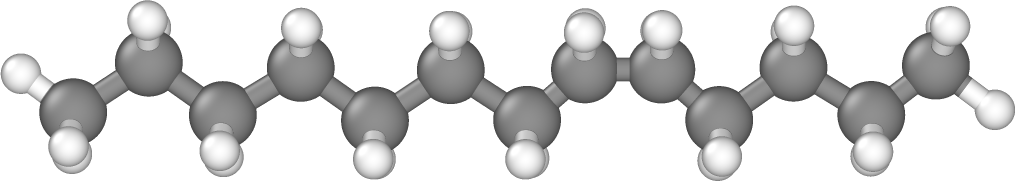
\includegraphics[width=0.8\linewidth]{Data/Images/RDF_Peaks.png}};
			%%%%

			\filldraw[fill=SERgray, draw=black]  	(6,2) circle (0.385*3/4) node {C};
			\filldraw[fill=SERwhite, draw=black]  	(5,2) circle (0.185) node {H};
			\draw node[] (d1_A) at (3.6,-0.5) {};
			\draw node[] (d1_B) at (4.92,-0.5) {};
			\draw node[] (d2_A) at (1.52,-0.5) {};
			\draw node[] (d3_A) at (1.4,1.99) {};
			\draw node[] (d3_B) at (2.89,1.59) {};
			\draw node[minimum width=10,minimum height=20,fill=white,rotate=53] (Cut1) at (0.069,0.85) {};
			\draw node[minimum width=10,minimum height=20,fill=white,rotate=53] (Cut2) at (6.8359,0.45) {};

			\draw node[] (Cut1) at (0.0,0.5) {...};
			\draw node[] (Cut2) at (6.835,0.5) {...};

            \dimline[line style = {line width=0.7},extension start length=-0.35,extension end length=-0.35] {(d1_A)}{(d1_B)}{$d_1$};
            \dimline[line style = {line width=0.7},extension start length=-0.24,extension end length=0.0] {(d2_A)}{(d1_A)}{$d_3$};
            \dimline[line style = {line width=0.7},extension start length=0.54,extension end length=0.54] {(d3_A)}{(d3_B)}{$d_2$};

		\end{tikzpicture}

		\caption{Distances $d_1$, $d_2$ and $d_3$ between pairs of carbon atoms corresponding to the first three peaks of the radial distribution functions for all the systems. }
		\label{fig:RDF_Peaks}
	\end{center}
\end{figure}


%%%%%%%%%%%%%%%%%%%%%%%%%%%%%%%%%%%%%%%%%%%%%%%%%

\section{Conclusions}
\label{sec:Conc}

In the present article we compared the behaviour of alkanes of three different length confined into two smooth parallel haematite ($\text{Fe}_2\text{O}_3$) surfaces. The comparison was made during equilibration, while reaching steady state (under shear), and after steady state was reached in terms of the end-to-end distance and segmental orientation of the chains, and of the changes in friction and temperature.

We propose a method to ensure that systems are properly equilibrated consisting of three criteria. The first two, consist on verifying that there is convergence of the mean squared end-to-end distance $\left(\left< R^2 \right> \right)$ and of  the mean squared radius of gyration $\left(\left< S^2 \right> \right)$.The last criterion, consists on following the mean squared displacement per atom $\left(\text{MSD}_{\text{atom}}\right)$ and per centre of mass of polymer chain $\left(\text{MSD}_{\text{CG}}\right)$ until the chains have moved --at least-- their own size\cite{Auhl2003}. All the systems equilibrated in such a way, show the formation of a  layered structure close to the surfaces; the polymer chains that are farther away  from the walls tend to form an amorphous-like region. 

For systems under shear, we propose to monitor the evolution of the mean squared end-to-end distance $\left(\left< R^2 \right> \right)$ and the segmental orientation $\left(\left<P_{2}^{xz} \right> \right)$ as representative parameters to determine when steady state has been attained. Our simulations  agree with previous experimental work that suggest\cite{Drummond2000} that the  evolution to steady-state sliding in thin films is governed by the distance the surfaces are sheared rather than the time.

From the point of view of the morphology of the polymer chains, we notice that, after reaching steady state, higher shearing velocities result in more compact (less elongated) molecules, and that longer chains tend to  lye  with a smaller angle with respect to the shearing direction.  We also see that the segmental orientation has a stronger dependency on the shearing velocity and on the chain length, than on the applied pressure.

In terms of the frictional response, we corroborate that higher pressures result on higher lateral (friction) forces, consistent with Amontons' first law for dry friction. Results also show that longer chains generate more friction than shorter chains by  generating larger amounts of viscous drag and that at higher velocities the  lateral (friction) force is almost independent of the chain length. Finally, we see that the high shearing velocities that we studied, for lower pressures, and especially for shorter chains, the lateral (friction) force remains constant independent of the velocity.

The friction coefficients are rather high, owing to solidification of the n-alkanes at the high contact pressure.

Friction higher than in previous simulations of thinner alkane films - no slip.

Friction much higher than in similar sized branched alkanes - solidification. Branched alkanes higher viscosity - but suppress crystalisation - lower EHL friction.

The shear stress increases with increasing chain length, but the differences are only significant at low speed.

The shear stress is far more sensitive to pressure than chain length in the range studied. At low pressure, the usual increase in shear stress with sliding velocity is observed. 

%%%%%%%%%%%%%%%%%%%%%%%%%%%%%%%%%%%%%%%%%%%%%%%%%
%%%%%%%%%%%%%%%%%%%%%%%%%%%%%%%%%%%%%%%%%%%%%%%%%
\section*{Acknowledgments}

S.E.R. acknowledges the support of the European Commission through the Marie Curie Industry-Academia Partnerships and Pathways (IAPP) iBETTER Project: \url{http://cordis.europa.eu/project/rcn/109976_en.html}. J.P.E acknowledges the financial support of the Engineering and Physical Sciences Research Council (EPSRC) via a Doctoral Prize Fellowship. D.D. also thanks the EPSRC for an Established Career Fellowship EP/N025954/1 and grant EP/P030211/1. All the figures of the atomic configurations where generated using the OVITO\cite{Stukowski2010b} software. Simulations were facilitated through the Imperial College London Research Computing Service (RCS).

%%%%%%%%%%%%%%%%%%%%%%%%%%%%%%%%%%%%%%%%%%%%%%%%%
%%%%%%%%%%%%%%%%%%%%%%%%%%%%%%%%%%%%%%%%%%%%%%%%%
%%%%%%%%%%%%%%%%%%%%%%%%%%%%%%%%%%%%%%%%%%%%%%%%%

% \begin{figure*}
%     	\begin{center}
% 		\begin{tikzpicture}
% 			\node[anchor=south west,inner sep=0] (fig_All_M_Profiles) at (0,0){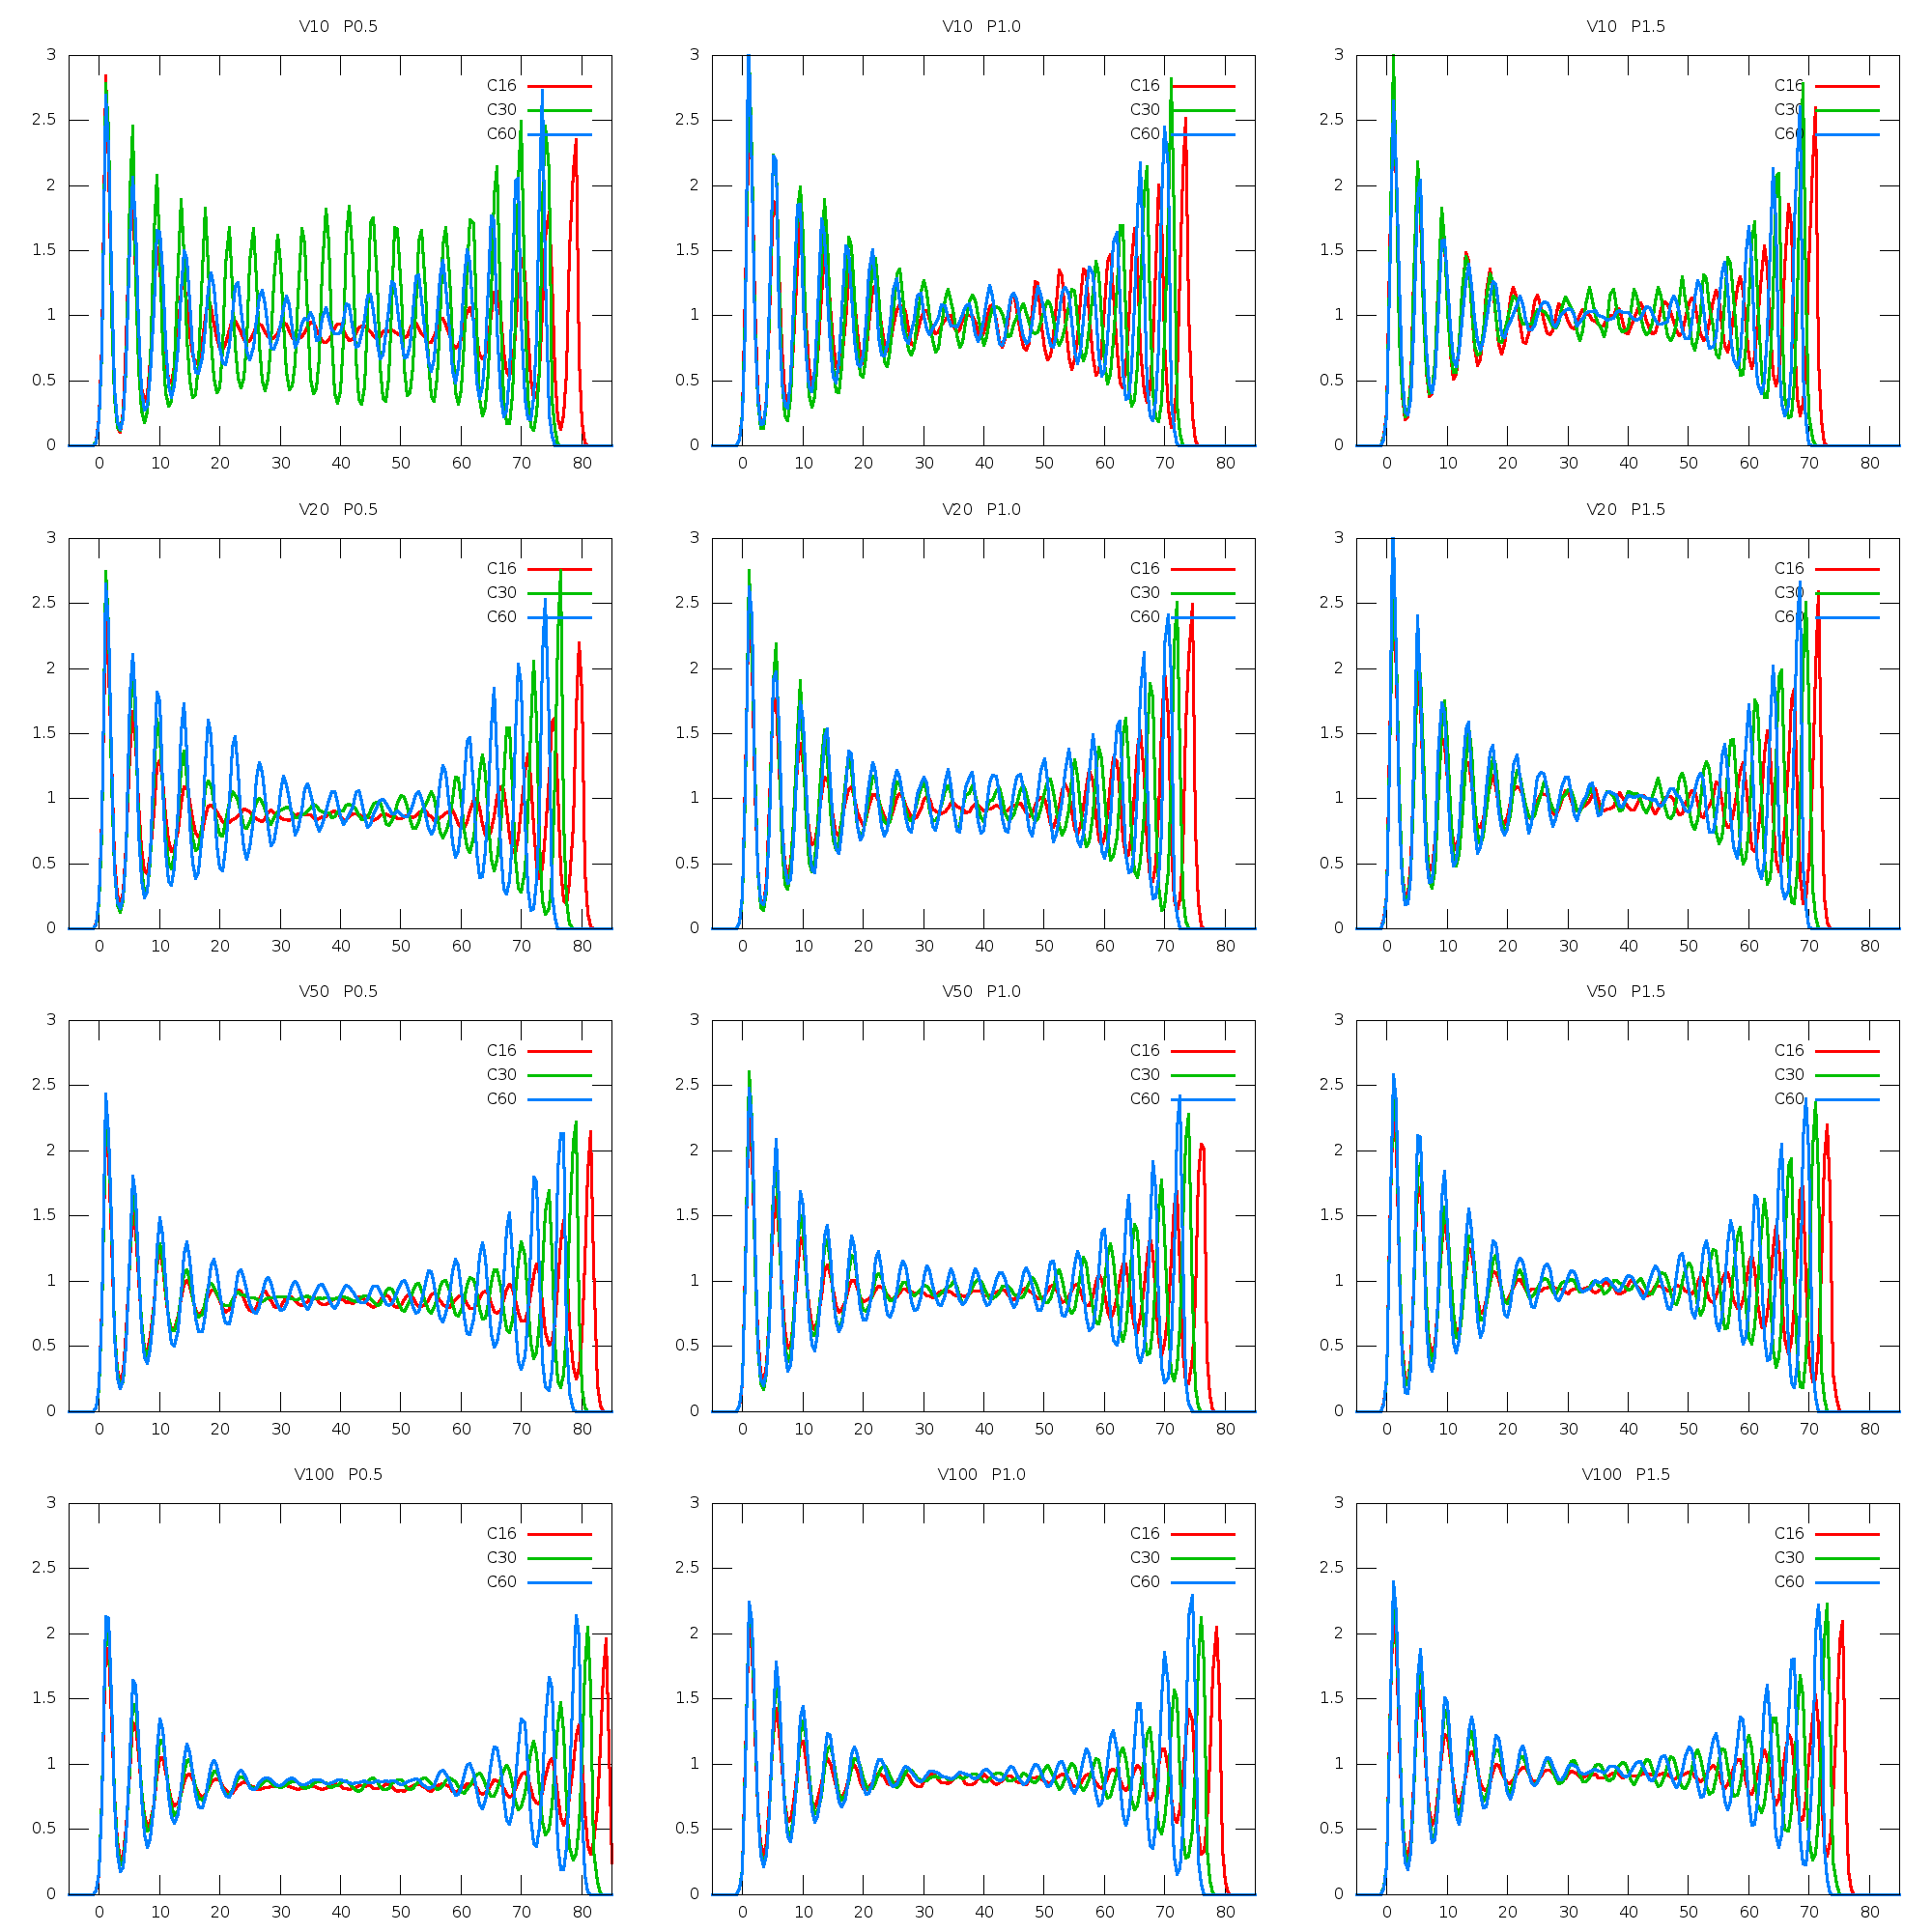
\includegraphics[width=\textwidth]{Data/Images/All_M_Profiles.png}};
% 			\begin{scope}[x={(fig_All_M_Profiles.south east)},y={(fig_All_M_Profiles.north west)}]
% 			\end{scope}
% 		\end{tikzpicture}
% 		\caption{}
% 		\label{fig:All_M_Profiles}
% 	\end{center}
% \end{figure*}

% \begin{figure*}
%     	\begin{center}
% 		\begin{tikzpicture}
% 			\node[anchor=south west,inner sep=0] (fig_All_RPF_Profiles) at (0,0){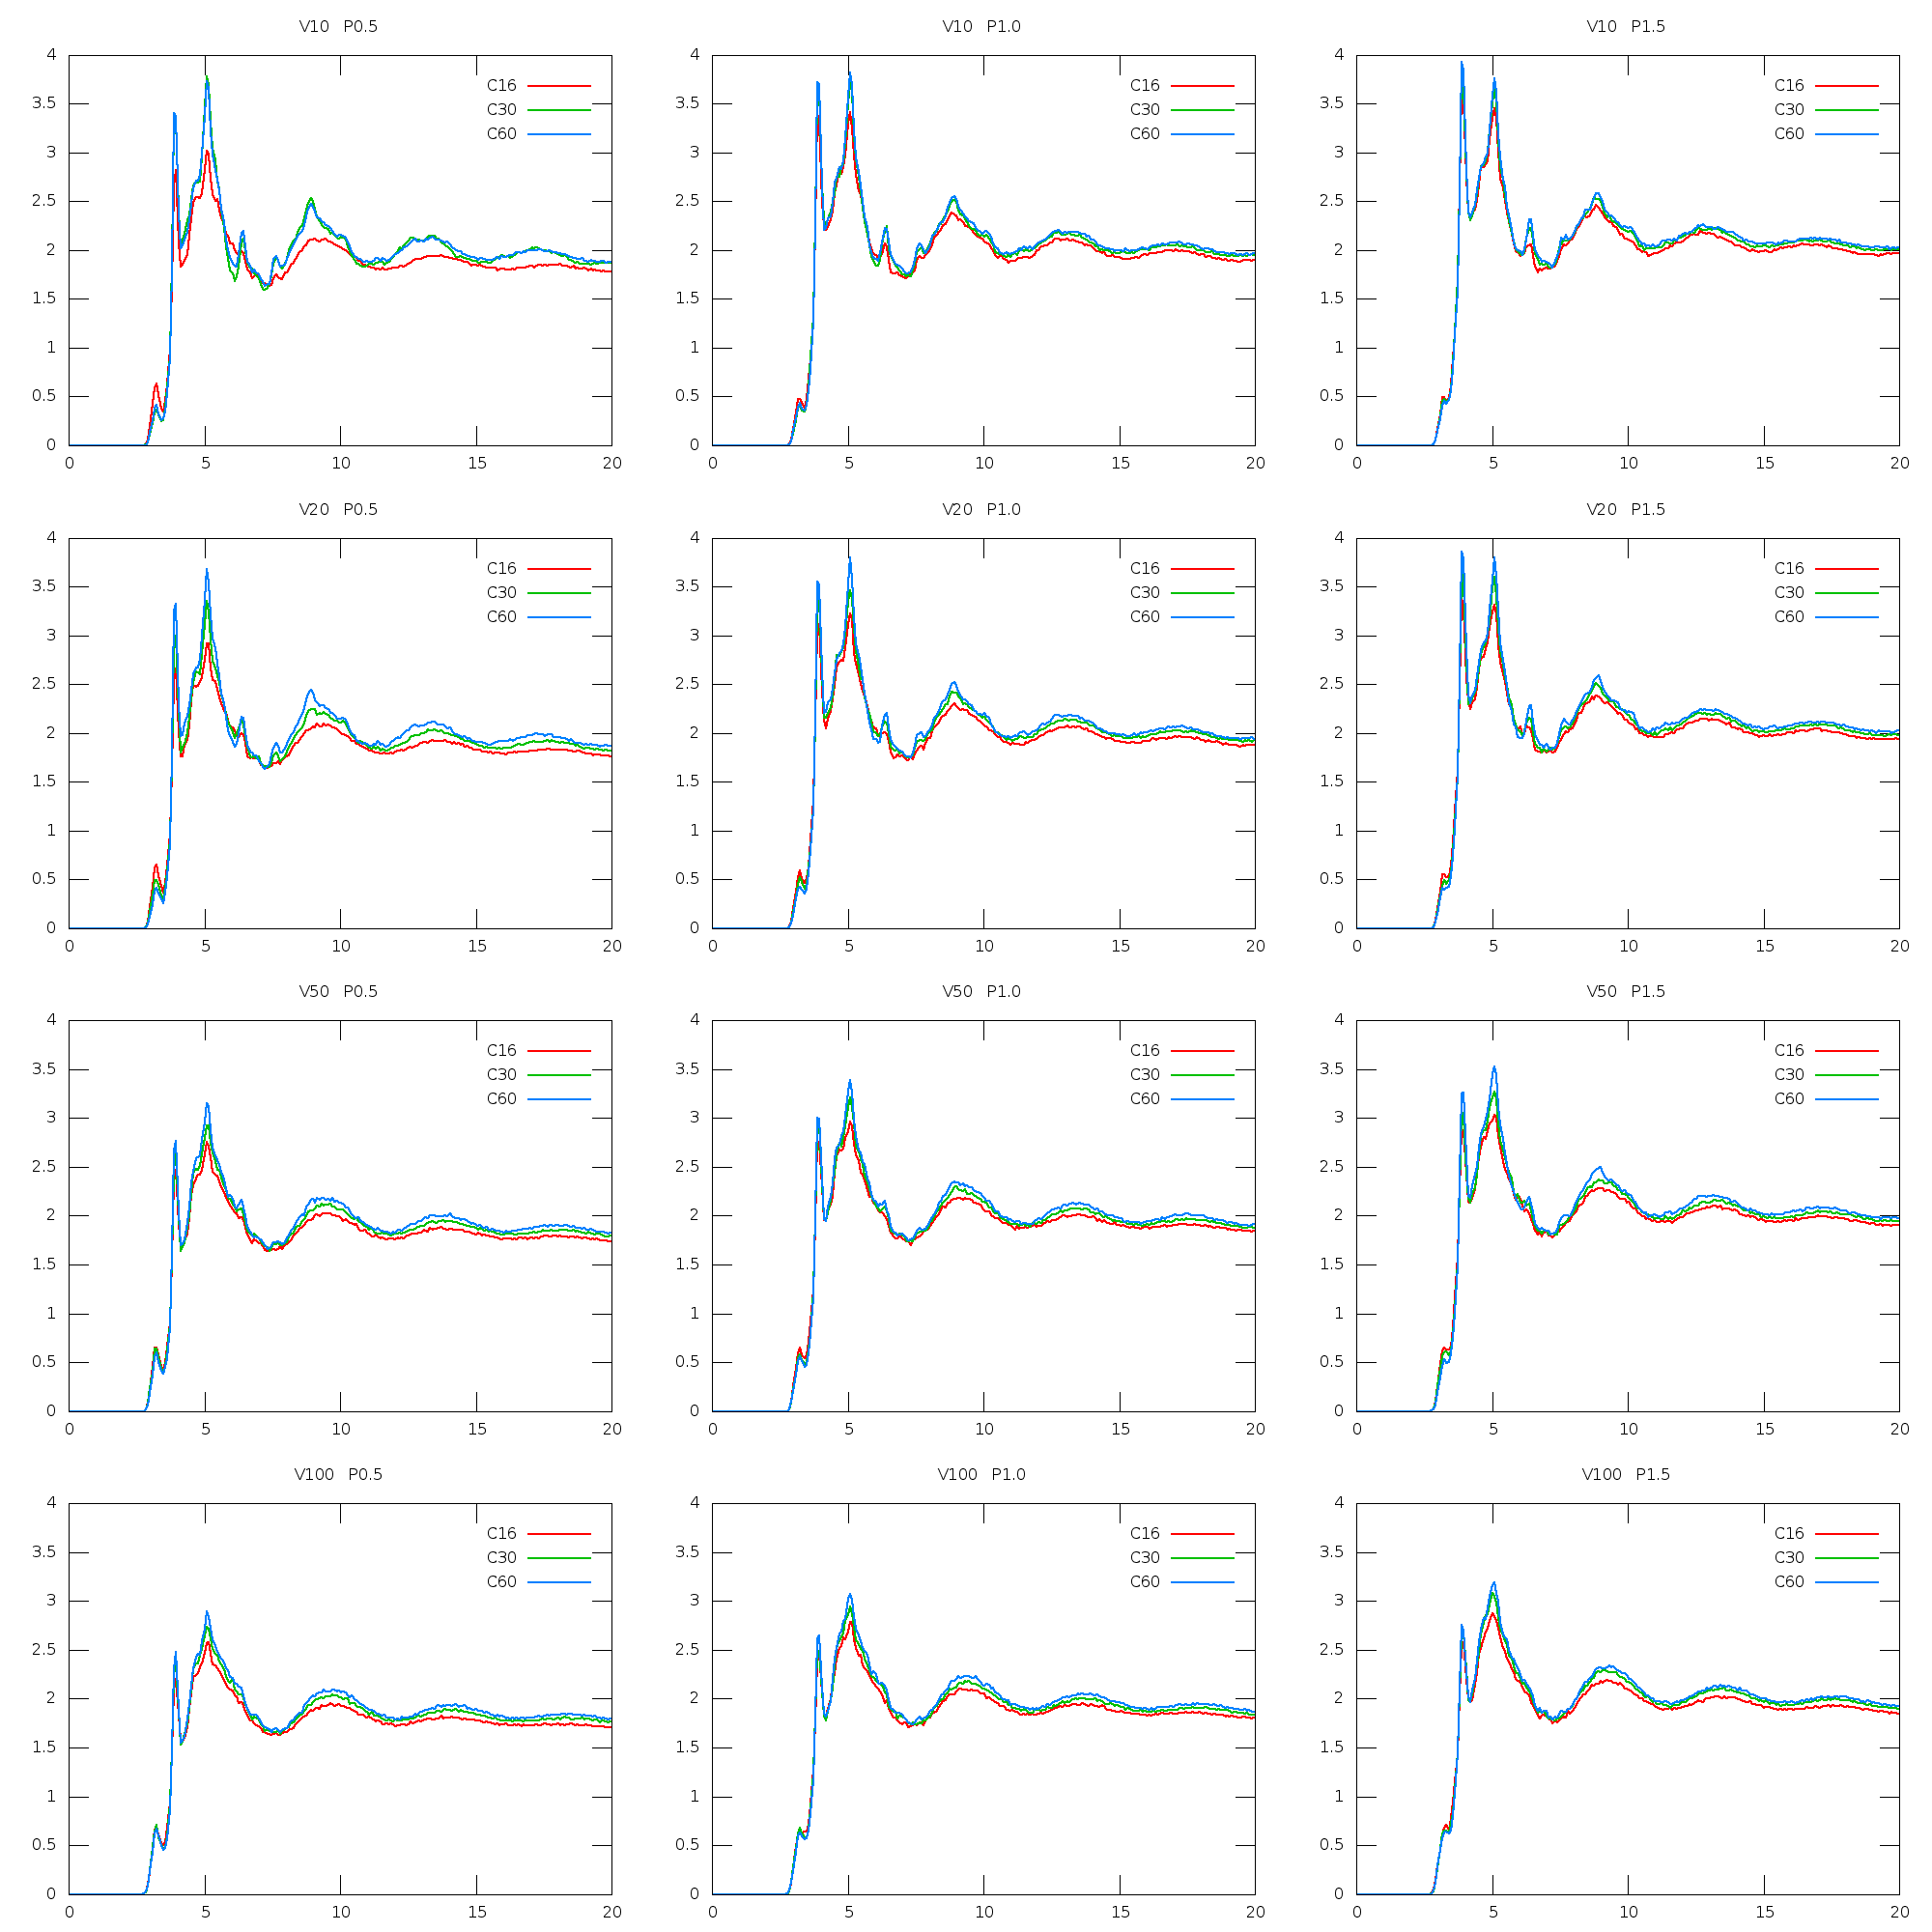
\includegraphics[width=\textwidth]{Data/Images/All_RPF_Profiles.png}};
% 			\begin{scope}[x={(fig_All_RPF_Profiles.south east)},y={(fig_All_RPF_Profiles.north west)}]
% 			\end{scope}
% 		\end{tikzpicture}
% 		\caption{}
% 		\label{fig:All_RPF_Profiles}
% 	\end{center}
% \end{figure*}

% \begin{figure*}
%     	\begin{center}
% 		\begin{tikzpicture}
% 			\node[anchor=south west,inner sep=0] (fig_All_T_Profiles) at (0,0){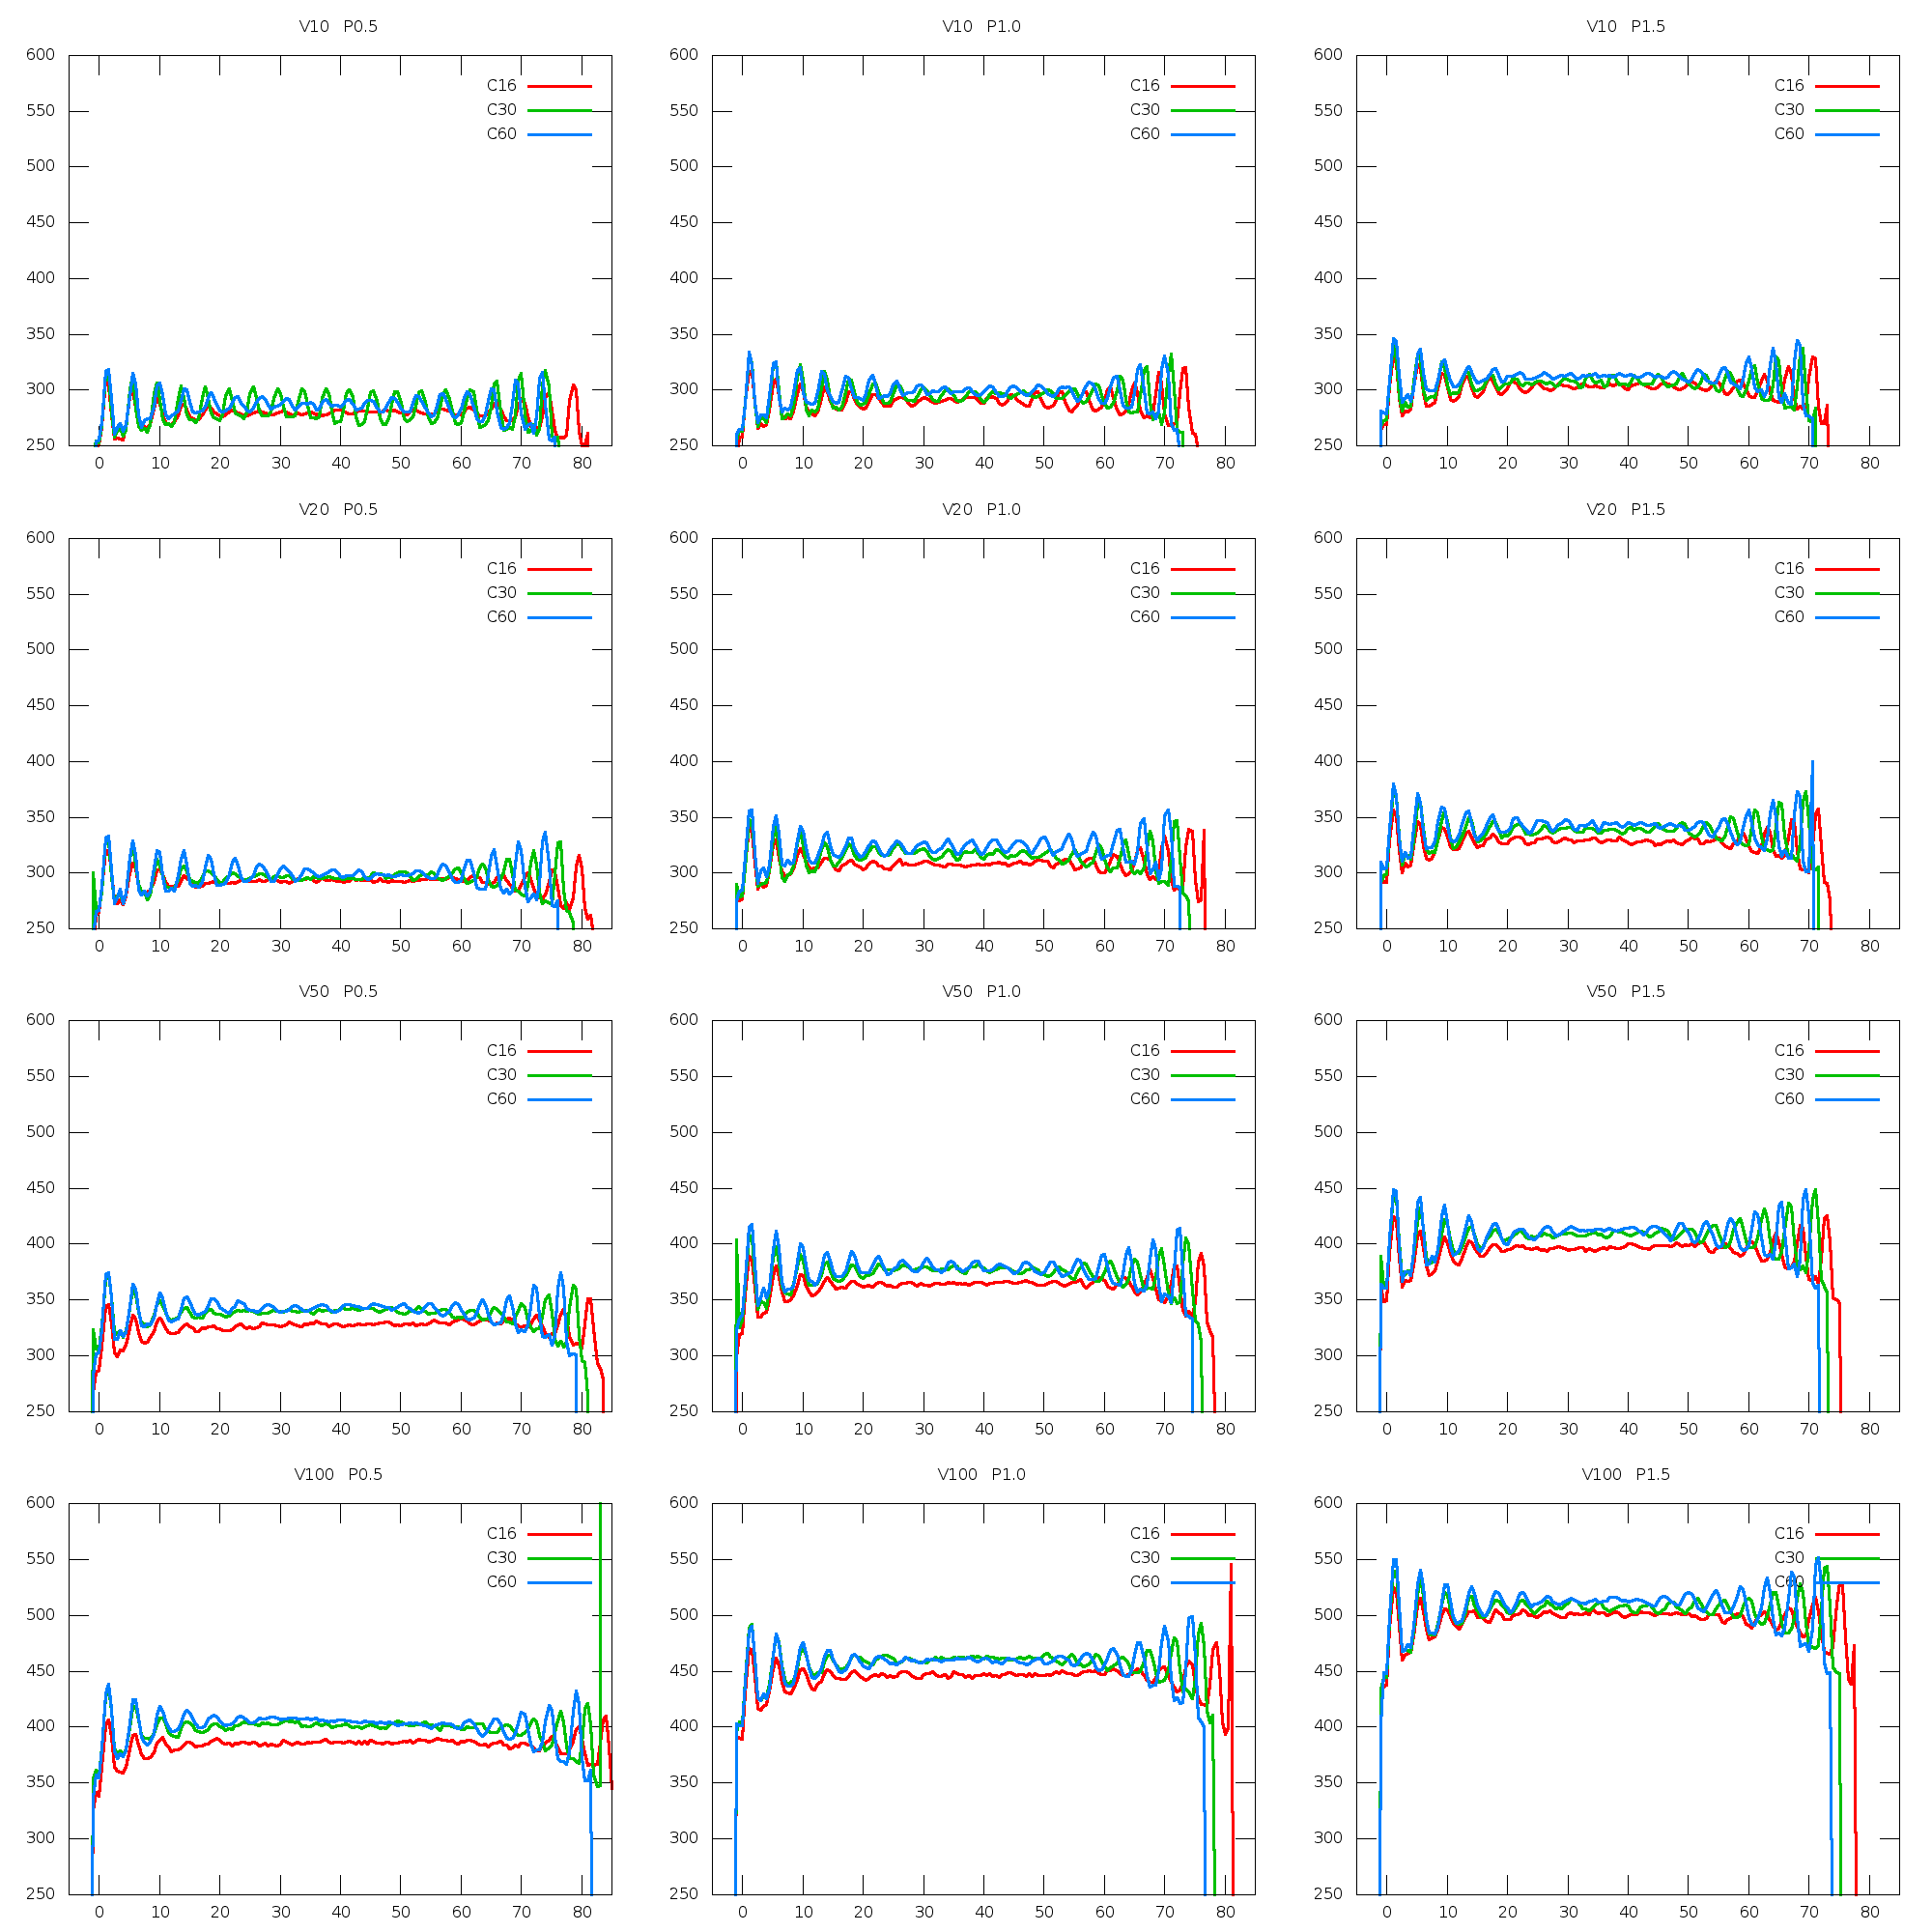
\includegraphics[width=\textwidth]{Data/Images/All_T_Profiles.png}};
% 			\begin{scope}[x={(fig_All_T_Profiles.south east)},y={(fig_All_T_Profiles.north west)}]
% 			\end{scope}
% 		\end{tikzpicture}
% 		\caption{}
% 		\label{fig:All_T_Profiles}
% 	\end{center}
% \end{figure*}

% \begin{figure*}
%     	\begin{center}
% 		\begin{tikzpicture}
% 			\node[anchor=south west,inner sep=0] (fig_All_V_Profiles) at (0,0){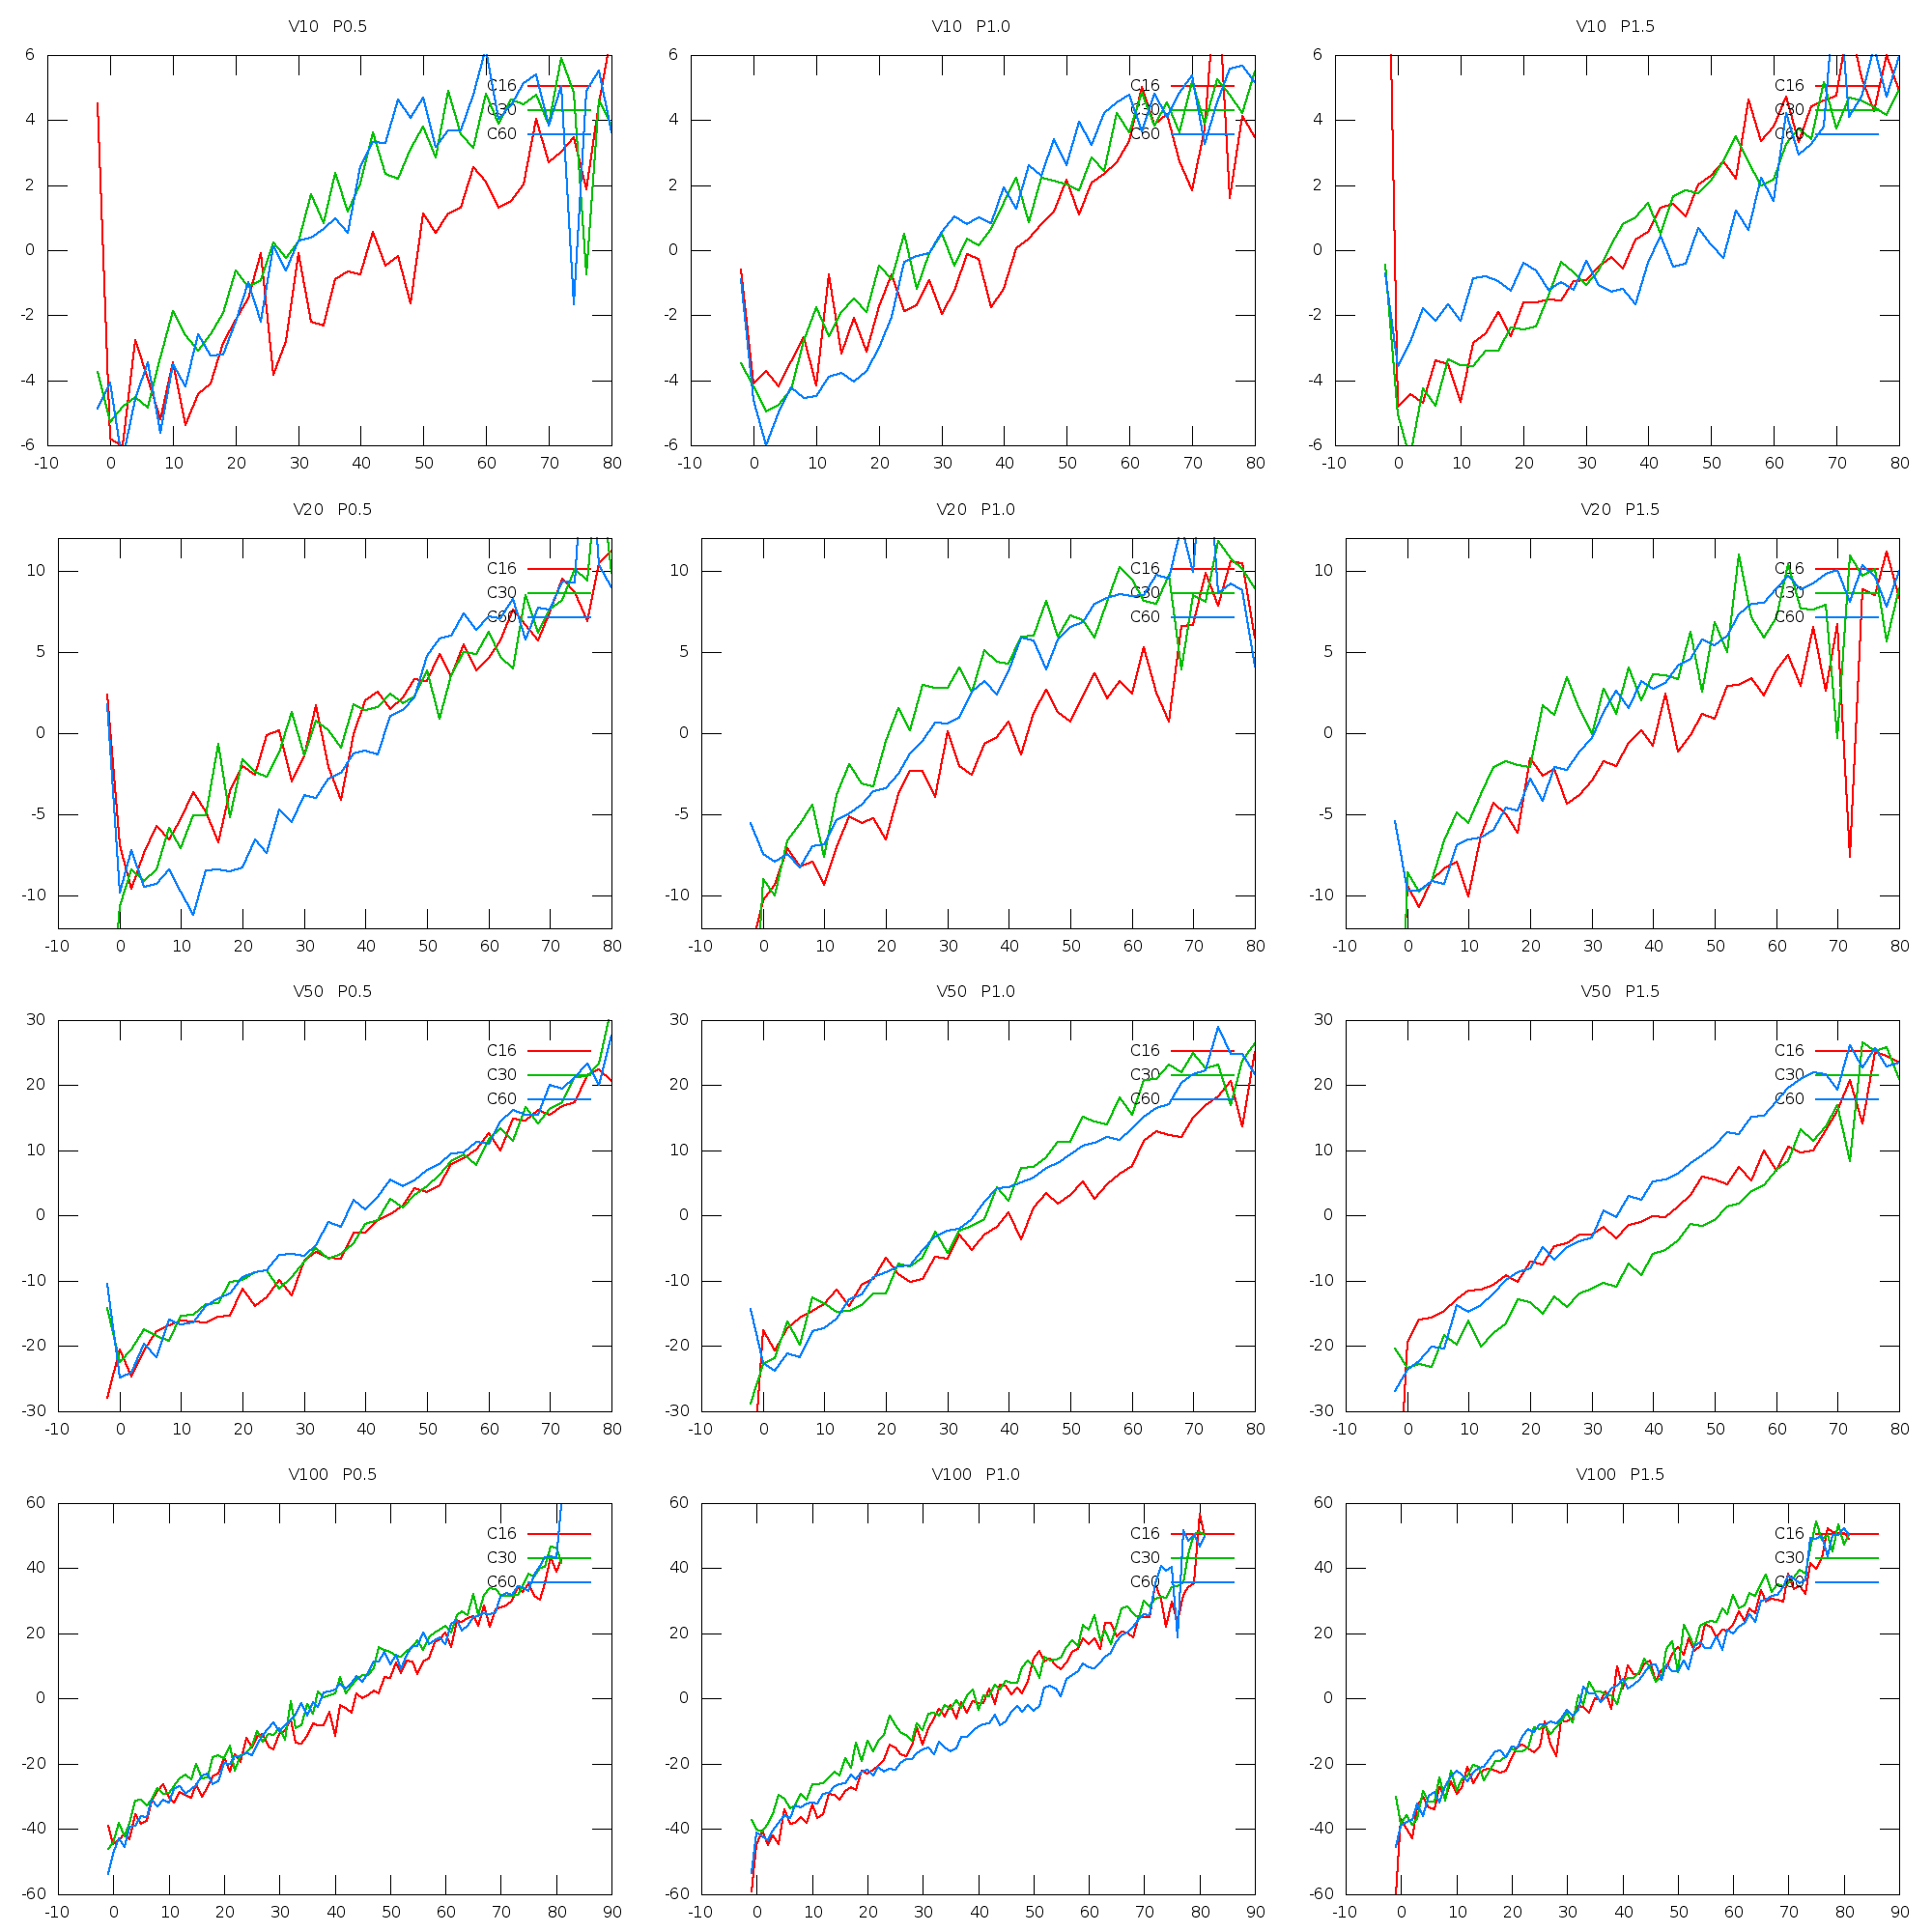
\includegraphics[width=\textwidth]{Data/Images/All_V_Profiles.png}};
% 			\begin{scope}[x={(fig_All_V_Profiles.south east)},y={(fig_All_V_Profiles.north west)}]
% 			\end{scope}
% 		\end{tikzpicture}
% 		\caption{}
% 		\label{fig:All_V_Profiles}
% 	\end{center}
% \end{figure*}

\appendix

\section{Equilibration}
The evolution of $\left< R^2 \right>$ and   $\left< S^2 \right>$  for C16, C30 and C60 at \SI{2000}{\kelvin} are presented on the main part of Figures  \ref{fig:e2e2} and \ref{fig:rg2}. For the case of the longest chains, which are the ones with lower diffusivity, these two quantities converge after approximately \SI{2e5}{} steps (\SI{0.2}{\nano\second}). The insets of the figures show the evolution of the same quantities but after reducing the temperature to \SI{353}{\kelvin}; we notice that after \SI{1e7}{} steps (\SI{10}{\nano\second}), both $\left(\left< R^2 \right> \right)$ and   $\left(\left< S^2 \right> \right)$ have reached their equilibrium values for the three  chain lengths considered. 

%\begin{gnuplot}[terminal=pdf]
%\end{gnuplot}

\pgfmathsetmacro{\SERFigwidth}{.035\linewidth}
\pgfmathsetmacro{\SERFigheight}{.026\linewidth}
\begin{figure}
    	\begin{center}
		\begin{gnuplot}[terminal=pdf, terminaloptions={size \SERFigwidth cm, \SERFigheight cm color solid}]
			set multiplot
			#set format x  '$10^{%L}$' 
			set format y  '$10^{%L}$' 
			#set format x  '%3.1e' 
			#set format y  '%3.1e' 
			set key top left
			set xlabel "Time [\\SI{}{\\nano\\second}]"  
			set ylabel "$\\left< R^2 \\right>  [\\SI{}{\\square\\angstrom}]$"
			set logscale x
			set logscale y
			set key noautotitle
			  plot  [1e-2:1e1] [:1e5]	'Data/Equilibration/C16/e2e2.plot' u ($1/1e6):($2) title 'C16' ,\
						'Data/Equilibration/C30/e2e2.plot' u ($1/1e6):($2)  title 'C30' ,\
						'Data/Equilibration/C60/e2e2.plot' u ($1/1e6):($2)  title 'C60'

			set origin 0.4,0.55
			set size 0.54,0.4
			unset xlabel
			unset ylabel
			set xtics(10, 15, 20)
			#set xtics ('$10^1$' 1e1,  '$1.5\mkern-5mu\times\mkern-5mu 10^1$' 1.5e1, '$2\mkern-5mu\times\mkern-5mu 10^1$' 2e1)
			set ytics font ',80'
			plot [1e1:2e1][]	'Data/Equilibration/C16/e2e2.plot' u ($1/1e6):($2) ,\
							'Data/Equilibration/C30/e2e2.plot' u ($1/1e6):($2) ,\
							'Data/Equilibration/C60/e2e2.plot' u ($1/1e6):($2) 
			unset multiplot
		\end{gnuplot}
		\caption{Evolution of the mean squared end-to-end distance $\left(\left< R^2 \right>\right)$ during the equilibration stage for the three considered alkane lengths: C16, C30 and C60. The main plot shows the initial equilibration at  \SI{2000}{\kelvin}; the inset the continuation at \SI{353}{\kelvin}. Note that $1 \times 10^{6}$ steps correspond to \SI{1}{\nano\second}.}
		\label{fig:e2e2}
	\end{center}
 \end{figure}


\pgfmathsetmacro{\SERFigwidth}{.035\linewidth}
\pgfmathsetmacro{\SERFigheight}{.026\linewidth}
\begin{figure}
    	\begin{center}
		\begin{gnuplot}[terminal=pdf, terminaloptions={size \SERFigwidth cm, \SERFigheight cm color solid}]
			set multiplot
			#set format x  '$10^{%L}$' 
			set format y  '$10^{%L}$' 
			set key top left
			set xlabel "Time [\\SI{}{\\nano\\second}]"  
			set ylabel "$\\left< S^2 \\right>  [\\SI{}{\\square\\angstrom}]$"
			set logscale x
			set logscale y
			set key noautotitle
			plot   [1e-2:1e1] [:1e4]	'Data/Equilibration/C16/Rg2.plot'  u ($1/1e6):($2) title 'C16' ,\
						'Data/Equilibration/C30/Rg2.plot'  u ($1/1e6):($2) title 'C30' ,\
						'Data/Equilibration/C60/Rg2.plot'  u ($1/1e6):($2) title 'C60'
			set origin 0.4,0.55
			set size 0.54,0.4
			unset xlabel
			unset ylabel
			set xtics(10, 15, 20)
			#set xtics ('$10^7$' 1e7,  '$1.5\mkern-5mu\times\mkern-5mu 10^7$' 1.5e7, '$2\mkern-5mu\times\mkern-5mu 10^7$' 2e7)
			set ytics font ',80'
			plot [1e1:2e1][]	'Data/Equilibration/C16/Rg2.plot' u ($1/1e6):($2) ,\
							'Data/Equilibration/C30/Rg2.plot' u ($1/1e6):($2) ,\
							'Data/Equilibration/C60/Rg2.plot' u ($1/1e6):($2) 
			unset multiplot
		\end{gnuplot}
		\caption{Evolution of the mean squared radius of gyration $\left(\left< S^2 \right>\right)$  during the equilibration stage for the three considered alkane lengths: C16, C30 and C60. The main plot shows the initial equilibration at \SI{2000}{\kelvin}; the inset the continuation at  \SI{353}{\kelvin}. Note that $1 \times 10^{6}$ steps correspond to  \SI{1}{\nano\second}.}
		\label{fig:rg2}
	\end{center}
 \end{figure}

The last criterion, is based on the fact that systems of long chain alkanes that are not properly equilibrated can present deformation on short length scales, and this deformation is only relaxed after the chains have moved at least their own size\cite{Auhl2003}. In order to verify this, the mean squared displacement per atom $\left(\text{MSD}_{\text{atom}}\right)$ and per centre of mass of alkane chain $\left(\text{MSD}_{\text{CG}}\right)$ are followed during equilibration. 

Figure \ref{fig:msd} shows the  $\text{MSD}_{\text{atom}}$ and $\text{MSD}_{\text{CG}}$ for the three different systems. Just like in the two previous figures, the main plot is dedicated to the evolution at  \SI{2000}{\kelvin}. Note that due to the artificial way that the chains are first introduced into the system (see Figure \ref{fig:Steps}), the diffusivity of the longer chains is initially higher than that of the shorter chains.  If we take the length of a C60 chain to be approx. \SI{74}{\angstrom} (the angle between the C-C bonds is \SI{109.5}{\degree} and the C-C distance equal to \SI{1.54}{\angstrom}),  it can be seen that the chains move their own size after approx. \SI{3e6}{} to  \SI{4e6}{} steps (\SI{3}{\nano\second} to \SI{4}{\nano\second}). Taking a conservative approach, the systems are equilibrated during  \SI{1e7}{} steps (\SI{10}{\nano\second}). The insets show the evolution after the temperature has been decreased; here, as expected, the slope of the $\text{MSD}_{\text{atom}}$ and $\text{MSD}_{\text{CG}}$ curves is shallower than at higher temperatures. 

\pgfmathsetmacro{\SERFigwidth}{.035\linewidth}
\pgfmathsetmacro{\SERFigheight}{.026\linewidth}
\begin{figure}
    	\begin{center}
		\begin{gnuplot}[terminal=pdf, terminaloptions={size \SERFigwidth cm, \SERFigheight cm color solid}]
			set multiplot
			#set format x  '$10^{%L}$' #'10^{%L}'
			set format y  '$10^{%L}$' #'10^{%L}'
			set xlabel "Time [\\SI{}{\\nano\\second}]"  
			set ylabel "$\\text{MSD}  [\\SI{}{\\square\\angstrom}]$"
			set key at 1.0e1, 1e3
			set logscale x
			set logscale y
			set key noautotitle
			plot [1e-2:1e1][1e2:] 	'Data/Equilibration/C16/msd.plot' 	 u ($1/1e6):($2) lc 1 pt 4 title 'C16',\
			   			'Data/Equilibration/C30/msd.plot' 			 u ($1/1e6):($2) lc 2 pt 4 title 'C30',\
			   			'Data/Equilibration/C60/msd.plot' 			 u ($1/1e6):($2) lc 3 pt 4 title 'C60'
			set origin 0,0
			set size 1,1

			set key at 1.5e1, 1e3
			plot [1e-2:1e1][1e2:]	'Data/Equilibration/C16/msd_cg.plot'  u ($1/1e6):($2)  lc 1 pt 7 title '  ',\
			   			'Data/Equilibration/C30/msd_cg.plot' 		  u ($1/1e6):($2)  lc 2 pt 7 title '  ',\
			   			'Data/Equilibration/C60/msd_cg.plot' 		  u ($1/1e6):($2)  lc 3 pt 7 title '  '

			set origin 0.145,0.55
			set size 0.54,0.4
			unset xlabel
			unset ylabel
			set xtics(10, 15, 20)
			#set xtics ('$10^7$' 1e7,  '$1.5\mkern-5mu\times\mkern-5mu 10^7$' 1.5e7, '$2\mkern-5mu\times\mkern-5mu 10^7$' 2e7)
			set ytics font ',80'
			plot [1e1:2e1][]	'Data/Equilibration/C16/msd.plot'  u ($1/1e6):($2) every 50 lc 1 pt 4 ,\
							'Data/Equilibration/C30/msd.plot'  u ($1/1e6):($2) every 50  lc 2 pt 4,\
							'Data/Equilibration/C60/msd.plot'  u ($1/1e6):($2) every 50  lc 3 pt 4,\
							'Data/Equilibration/C16/msd_cg.plot'  u ($1/1e6):($2) every 50  lc 1 pt 7,\
							'Data/Equilibration/C30/msd_cg.plot'  u ($1/1e6):($2) every 50  lc 2 pt 7,\
							'Data/Equilibration/C60/msd_cg.plot'  u ($1/1e6):($2) every 50  lc 3 pt 7


			unset multiplot
		\end{gnuplot}
		\caption{Evolution of the mean squared displacement (MSD) during the equilibration stage for the three considered alkane lengths: C16, C30 and C60. The main plot shows the initial equilibration at  \SI{2000}{\kelvin}; the inset the continuation at  \SI{353}{\kelvin}. The full circles represent the mean squared displacement per atom $\left(\text{MSD}_{\text{atom}}\right)$ while the empty squares the mean squared displacement per centre of mass of polymer chain $\left(\text{MSD}_{\text{CG}}\right)$. Note that $1 \times 10^{6}$ steps correspond to  \SI{1}{\nano\second}.}
		\label{fig:msd}
	\end{center}
 \end{figure}



\bibliography{MyCollection}
\bibliographystyle{unsrt}

\end{document}


%%%%%%%%%%%%%%%%%%%%%%%%%%%%%%%%%%%%%%%%%%%%%%%%%

\section{Supplementary Information}

\subsubsection{Segmental Orientation}

Particle models like MD allow to measure orientation of polymer segments explicitly by taking the orientation of a bond as a segment orientation. The segmental orientation \cite{Monnerie1983,Erman1985,Besbes1992} of the fluid in terms of the second Legendre polynomial $\left(P_2\right)$ is defined as:

\begin{equation}\label{eq:P_2}
\left\langle P_2 \right\rangle =\frac{3\left\langle \cos ^2 \alpha \right\rangle - 1}{2},
\end{equation}

where $\alpha$ is the angle between a chain segment and a reference axis. In practice, $\left\langle \cos ^2 \alpha \right\rangle$ is calculated in the following way:

\begin{equation}
\left\langle \cos ^2 \alpha \right\rangle = \frac{1}{N_\text{bonds}} \sum_{b=1}^{N_\text{bonds}} \left(\frac{\textbf{r}^b_{ij}}{r^b_{ij}} \cdot \mathbf{\hat \imath} \right)^2
\end{equation}

 in which $N_\text{bonds}$ is the total number of bonds, $\textbf{r}^b_{ij}$ is the difference between the positions of the two beads that form the bond $b$, and $\mathbf{\hat \imath}$ is the direction of the main axis. 
 
 In this work we are interested in  the changes of the orientation in the shearing direction, so we will only focus on  the segmental orientation with respect to $x$ projected in the $xz$ plane: $P_{2}^{xz}$. Note that, by definition,  if all the chains are parallel to the shearing direction $\langle P_{2}^{xz}\rangle=1 $; if all the chains are perpendicular to the surfaces   $\langle P_{2}^{xz} \rangle=-0.5$, and, interestingly, if all the chains are oriented at  \SI{45}{\degree} or if they are randomly oriented $\langle P_{2}^{xz}\rangle=0.25 $
 
%%%%%%%%%%%%%%%%%%%%%%%%%%%%%%%%%%%%%%%%%%%%%%%%%

\subsubsection{Mean squared end-to-end distance}

The  squared end-to-end distance  of a single polymer chain is defined as the square  of the magnitude of  the vector that points from one end of a polymer to the other end. for a system containing several polymer chains, the mean squared end-to-end distance $\left(\left< R^2 \right>\right)$ is given by the following equation \cite{Brown1994}:

\begin{equation}
	\left< R^2 \right> = \left<\left( \mathbf{r}_1 - \mathbf{r}_N \right)^2\right>
	\label{eq:e2e2}
\end{equation}

where, for each polymer chain,  $N$ is the number of atoms and  $ \mathbf{r}_i$ is the position vector of atom $i$. 

%%%%%%%%%%%%%%%%%%%%%%%%%%%%%%%%%%%%%%%%%%%%%%%%%

\subsubsection{Mean squared radius of gyration}

The mean squared radius of gyration $\left(\left< S^2 \right>\right)$  is the average squared distance of each atom in the polymer chain  from its centre of mass, as defined in the following equation\cite{Brown1994}:

\begin{equation}
	\left< S^2 \right> = \frac{\left< \sum_{i=1}^{N}  \left ( \lVert \mathbf{r}_i - \mathbf{r}_{\text{com}} \rVert \right)^2 \right>}{N}
\end{equation}

where, for each polymer chain,  $N$ is the number of atoms, $ \mathbf{r}_i$ is the position vector of atom $i$  and $\mathbf{r}_{\text{com}}$ is the centre of mass. 

%%%%%%%%%%%%%%%%%%%%%%%%%%%%%%%%%%%%%%%%%%%%%%%%%

\subsubsection{Mean squared displacement}

The mean squared displacement (MSD) of an atom  is a measure of the deviation between its  current  and its initial position. For a material block consisting of several atoms, the  MSD averaged over the number of atoms  $\left(N\right)$ can be used to quantify  diffusion. The MSD is defined as:

\begin{equation}
	\text{MSD} = \frac{1}{N}\sum_{i=1}^{N} \left( \mathbf{r}_i\left(t\right)-\mathbf{r}_i\left(0\right)\right)^2
\end{equation}

where   $\mathbf{r}_i\left(t\right)$ is a vector containing the coordinates of atom $i$ at time $t$.


%%%%%%%%%%%%%%%%%%%%%%%%%%%%%%%%%%%%%%%%%%%%%%%%%

\subsubsection{Temperature}

As common in NEMD simualtions, the temperature of the lubricant is calculated via the kinetic energy of the atoms but excluding the velocity component in the direction of sliding (x) to avoid contributions that are not related to the thermal vibration of the atoms. The measurements are averaged every 100 steps to damp the fluctuations that are characteristic of the relatively small system size.

%%%%%%%%%%%%%%%%%%%%%%%%%%%%%%%%%%%%%%%%%%%%%%%%%
%%%%%%%%%%%%%%%%%%%%%%%%%%%%%%%%%%%%%%%%%%%%%%%%%
%%%%%%%%%%%%%%%%%%%%%%%%%%%%%%%%%%%%%%%%%%%%%%%%%


%git pull
%git add -A
%git commit
%git push origin master


